\chapter*{Rekonstruktionsverfahren und ihre Implementierung}
\label{cha:3}

In diesem Kapitel werden wir die praktische Vorgehensweise einiger Bildrekonstruktionstechniken in der Computertomographie diskutieren. Den Stützpunkt folgender Diskussion werden wir zuerst hier festigen. Dazu schauen wir uns nochmal das diskrete Modell (\ref{equa:2.2}) an:

\[\mathcal{R}f = \sum\limits_{j = 1}^{n} \sigma_j \langle f, v_j\rangle_{L^2(\Omega)} u_j, \ \ n \in \N.\] 

Die obige Gleichung stellt genau $n$ Projektionen $p \in \R^n$ einer unbekannten Dichtefunktion $f \in \R^m$ dar. Die Anzahl der Projektionen $n$ setzt sich aus der Anzahl der Detektorzellen $k \in  \N$ im Detektorband und der Anzahl der Winkel $q \in \N$ zu denen die Projektionen erzeugt worden sind zusammen. Insgesamt ergibt sich
\begin{equation}
	n = kq \ \ \mbox{für} \ n,k,q \in \N.
	\label{equa:3.1}
\end{equation}
\begin{figure}[H]
	\centering
	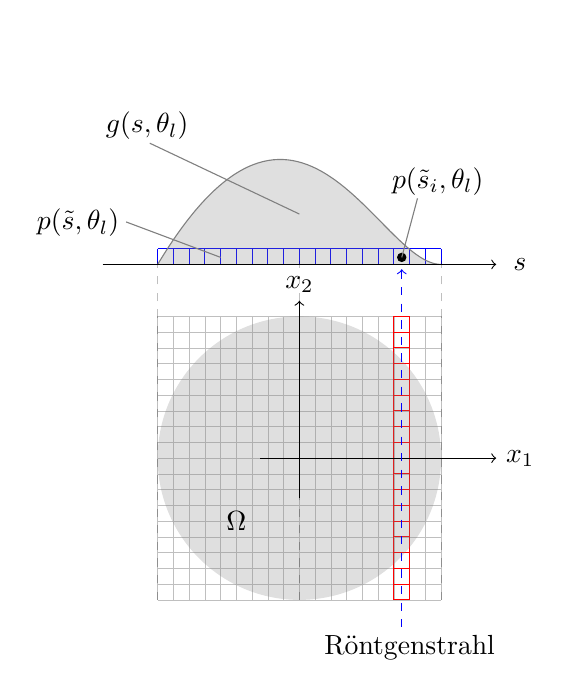
\begin{tikzpicture}
	
	\draw [step=0.2,blue, thin, rotate=0, xshift=0, yshift=70] (-1.8,0) grid (1.8,0.2); % detector grid
	
	\draw [step=0.2, lightgray, very thin] (-1.8,-1.8) grid (1.8,1.8); % picture grid
	
	\draw [step=0.2, red, thin, rotate=0, xshift=1.2cm, yshift=0] (0,-1.8) grid (0.2,1.8);
	
	\fill[nearly transparent, color=gray] (0,0) circle (1.8cm);
	
	\draw [black] [->](-0.5,0) -- (2.5,0); % x-Achse
	\draw [black] (2.5, 0) node [right] {$x_1$};
	
	\draw [black] [->](0,-0.5) -- (0,2); % y-Achse
	\draw [black] (0, 2.2) node {$x_2$};
	
	\draw [rotate=0, xshift=1.3cm, <-, dashed] [blue] (0,2.4) -- (0,-2.2); % strahl
	\draw [black] (1.4, -2.4) node {Röntgenstrahl};
	
	\draw [gray] [rotate=0, yshift=70] (-1.8,0) .. controls (0,3) and (1,0) .. (1.8,0);
	\fill [nearly transparent, color=gray] [rotate=0, yshift=70] (-1.8,0) .. controls (0,3) and (1,0) .. (1.8,0);
	
	\fill[ rotate=0, xshift=0cm, yshift=1.8cm, black](1.3,0.75) circle [radius=0.06]; % ein Punkt
	
	\draw [rotate=0, xshift=0, yshift=70] [black] [->] (-2.5,0) -- (2.5, 0);
	\draw [black] (2.8, 0)  node [rotate=0, xshift=0, yshift=70] {$s$};
	
	\draw [black] (0, 0)  node [rotate=0, xshift=-80, yshift=85] {$p(\tilde{s}, \theta_l)$};
	\draw[gray,  yshift=1.8cm](-1,0.75) -- (-2.2, 1.2);	
	
	\draw [black] (0, 0)  node [rotate=0, xshift=50, yshift=100] {$p(\tilde{s}_i, \theta_l)$};
	\draw[gray,  yshift=1.8cm](1.3,0.75) -- (1.5, 1.5);		
	
	\draw [black] (0, 0)  node [rotate=0, xshift=-55, yshift=120] {$g(s, \theta_l)$};
	\draw[gray,  yshift=1.8cm](0,1.3) -- (-1.9, 2.2);		
	
	\draw [rotate=0, xshift=0cm, dashed] [nearly transparent, color=black] (0,-1.8) -- (0,2.5); % punktiert Mitte
	\draw [rotate=0, xshift=1.8cm, dashed] [nearly transparent, color=black] (0,-1.8) -- (0,2.5); % rechts punktiert
	\draw [rotate=0, xshift=-1.8cm, dashed] [nearly transparent, color=black] (0,-1.8) -- (0,2.5); % links punktiert 
	
	\draw [black] (-0.8, -0.8) node {$\Omega$};
	
	\end{tikzpicture}
	\caption{Anschauliche Darstellung der Diskretisierung der Dichtefunktion $f$. Entlang des Röntgenstrahls (alle rot umrandeten Pixel) an der Stelle $s_i$ und zu einem festen Winkel $\theta_l = 0$, werden die Werte von $f$ zu dem Wert $p(\tilde{s}_i, \theta_l)$ aufsummiert. $p(\tilde{s}, \theta_l)$ ist der Vektor zu allen Strahlen an den Stellen $\tilde{s}_i$ und somit die Diskretisierung von $g(s,\theta_l)$.}
	\label{fig:3.1}
\end{figure}
Die Diskretisierung von $f$ hängt hingegen nur von der Anzahl der Detektorzellen $k \in \N$ im Detektorband ab. Betrachtet man die Abbildung \ref{fig:3.1}, dann wird man erkennen, dass die $k$ Detektorzellen die Breite und die Höhe des zu rekonstruierenden Bildes $f$ festlegen, demnach ergibt sich
\begin{equation}
	m = k^2 \ \ \mbox{für} \ k, m \in \N.
	\label{equa:3.2}
\end{equation}
\begin{Bemerkung}
	Praktisch gesehen, stellt $k$ die Anzahl der digitalen Pixel in der Breite und Tiefe eines digitalen Bildes $f$ dar.
	\label{bem:6}
\end{Bemerkung}
Bevor wir im nächsten Schritt zur Bildrekonstruktion übergehen, schauen wir uns zuerst die Entstehung der Projektionsdaten aus der Radon Transformation etwas genauer an. Betrachten wir dazu die Gleichung (\ref{equa:1.10}) und die Abbildung \ref{fig:1.6}.
\[ \mathcal{R}f(s,\theta) = \int\limits_{-\gamma(s)}^{\gamma(s)} f(s\omega(\theta) + t\omega^{\perp}(\theta))\mbox{d}t. \]
Im diskreten Fall $\tilde{f} \in \R^{k \times k}$ wird man feststellen, dass (\ref{equa:1.10}) die Summe aller Werte von $\tilde{f}$ entlang einer Geraden $G$, den Projektionswert $p(\tilde{s}_i, \theta_l)$ an der Stelle $\tilde{s}_i, i \in [1,k]$, entsprechend dem Winkel $\theta_l, \ l \in [1,q] $, liefert. Damit kann (\ref{equa:1.10}) für die Transformation eines digitalen Bildes folgendermaßen interpretiert werden
\begin{equation}
	\begin{split}
		p(\tilde{s}_i, \theta_l) & = \sum \limits_{j = 1}^{m} \mu_j \Delta\tilde{t}, \ \mbox{mit} \ m = k^2, \\
		\mbox{für} \ \mu_j & = \left\{ \begin{matrix}
							\tilde{f}_j & : & \mbox{falls } \tilde{f}_j\cap G \neq \emptyset \\ 
							0 & : & \mbox{sonst}
						\end{matrix}.\right.
	\end{split}
	\label{equa:3.3}
\end{equation}

Fasst man auf diese Weise zu jedem $\tilde{s}_i$ (wobei $\Delta\tilde{t} = 1$) die entsprechende Werte von $\tilde{f}$ zusammen, so entsteht der Projektionsvektor $p(\tilde{s},\theta_l)$ (Abb. \ref{fig:3.1}). Stellt man alle Projektionen $p(\tilde{s}, \theta_l)$ entsprechend der Winkelreihenfolge $\theta_l, \ l \in [1,q]$ auf, so entsteht ein digitales Bild der Projektionsdaten der diskreten Radon Transformation.
\begin{Bemerkung}
	Die Gleichung (\ref{equa:3.3}) entspricht der Parallelstrahlengeometrie. Das bedeutet, dass alle Geraden $G$, die das Objekt durchdringen, parallel zueinander sind. Um (\ref{equa:3.3}) in die Fächerstrahlengeometrie zu überführen, müssen entsprechende geometrische Transformationen durchgeführt werden.
	\label{bem:7}
\end{Bemerkung}

Schauen wir uns ein konkretes Beispiel einer Radon Transformation an. Sei dazu die Abbildung \ref{fig:3.2} betrachtet. In Abb. \ref{fig:3.2.b} ist die Radontransformierte oder \textit{das Sinogramm} von Abb. \ref{fig:3.2.a} gemäß (\ref{equa:3.3}) zu sehen. Der Aufbau des Sinogramms entspricht dem oben beschriebenen Prinzip. Fasst man also das Sinogramm in Abb. \ref{fig:3.2.b} als eine Matrix auf, so ist jede Spalte der Matrix gleich einer Projektion $g(\tilde{s}, \theta_l)$ zu einem festem Winkel $\theta_l$. Die Implementierung der (diskreten) Radon Transformation ist im Abschnitt \ref{cha:A.1} kurz erläutert.
\begin{figure}[H]
	\begin{center}
		\subfloat[\label{fig:3.2.a}Phantombild]{{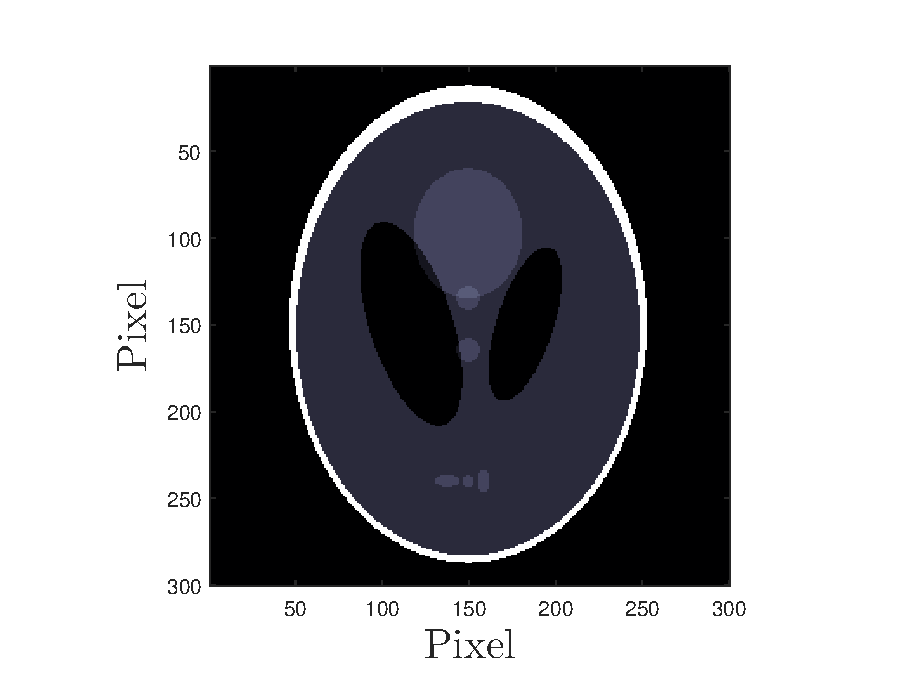
\includegraphics[width=0.5\textwidth]{phantom.eps} }}
		\subfloat[\label{fig:3.2.b}Die Radon Transformation des Phantombildes]{{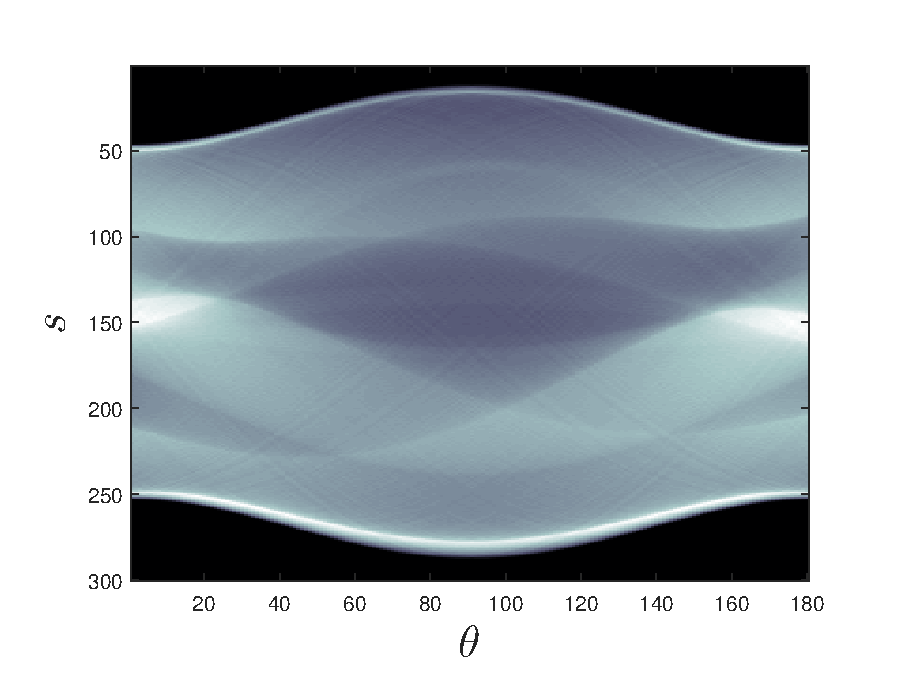
\includegraphics[width=0.5\textwidth]{rt_phantom.eps} }}
	\end{center}
	\caption{ Links (a) ist ein Phantombild (Quelle: \MATLAB, \texttt{\captionstring phantom(300)}) zu sehen, welches wir für alle Testzwecke in diesem Kapitel benutzen werden. Rechts (b) ist die Radontransformierte von (a) abgebildet. Die Transformation wurde über $\theta \in [0^{\circ}, 180^{\circ}]$ mit einer Schrittweite von $1^{\circ}$ durchgeführt. Das Detektorband hat eine Länge von $k = 300$, wobei $k$ gleich der Anzahl der Tiefenpixel von (a) ist. Somit bestimmt $k$ auch die Anzahl der Strahlen, die durch das Phantombild geschickt worden sind.}
	\label{fig:3.2}
\end{figure}

Sinogramme sind in der Praxis der computertomographischen Bildrekonstruktion genau die gemessenen Daten. Somit ist die Aufgabe das Bild des Ursprungsobjekts aus einem Sinogramm zu rekonstruieren. In folgenden Abschnitten werden wir uns vier solcher Rekonstruktionsverfahren anschauen. Dabei unterscheiden wir zwischen \textit{analytischen} und \textit{algebraischen} Verfahren. Als Nächstes wollen wir den Begriff der analytischen Rekonstruktion klären.

\section*{Analytische Rekonstruktionsverfahren}
\label{cha:3.1}

Der Begriff der \textit{analytischen Rekonstruktion} bedeutet in diesem Fall, dass die Algorithmen der CT-Bildrekonstruktion direkt aus den analytischen Formeln hergeleitet werden. Solche Verfahren nutzen die Projektionsdaten zur Rekonstruktion des Bildes direkt aus. Zuerst schauen wir uns das einfachste davon an.

\subsection*{Ungefilterte Rückprojektion}
\label{cha:3.1.1}

Den Ausgangspunkt dieses Abschnitts liefert uns der Adjungierte Operator (\ref{equa:1.21}). Schauen wir uns die Gleichung des Operators $\mathcal{R}^*$ noch einmal an: 

\[ \mathcal{R^*} g(x) = \int\limits_{0}^{\pi} \ g(x^{T}\omega(\theta),\theta) \mbox{d}\theta. \]  

Aus der Bemerkung \ref{bem:3} wissen wir bereits, dass (\ref{equa:1.21}) die ungefilterte Rückprojektion darstellt. Das Argument des Integranden in der obigen Gleichung ist ein fester Punkt $x$ der Kreisscheibe $\Omega$. Auf diesen Punkt $x$ wird aus allen Winkeln zurück projiziert. Führt man das für alle $x \in \Omega$ durch, so entsteht ein verschwommenes Bild des Originals, wie es die Abbildung \ref{fig:3.3.b} zeigt.
\begin{figure}[!h]
	\begin{center}
		\subfloat[\label{fig:3.3.a}Die Radon Transformation des Phantombildes aus Abb. \ref{fig:3.2.a}.]{{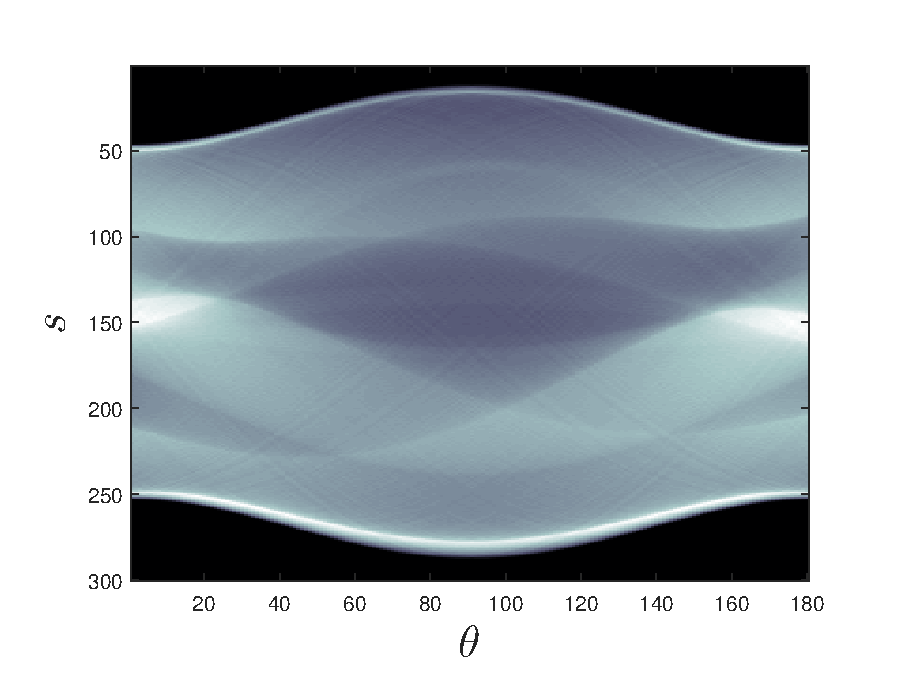
\includegraphics[width=0.5\textwidth]{rt_phantom.eps} }}
 		\subfloat[\label{fig:3.3.b}Ungefilterte Rückprojektion]{{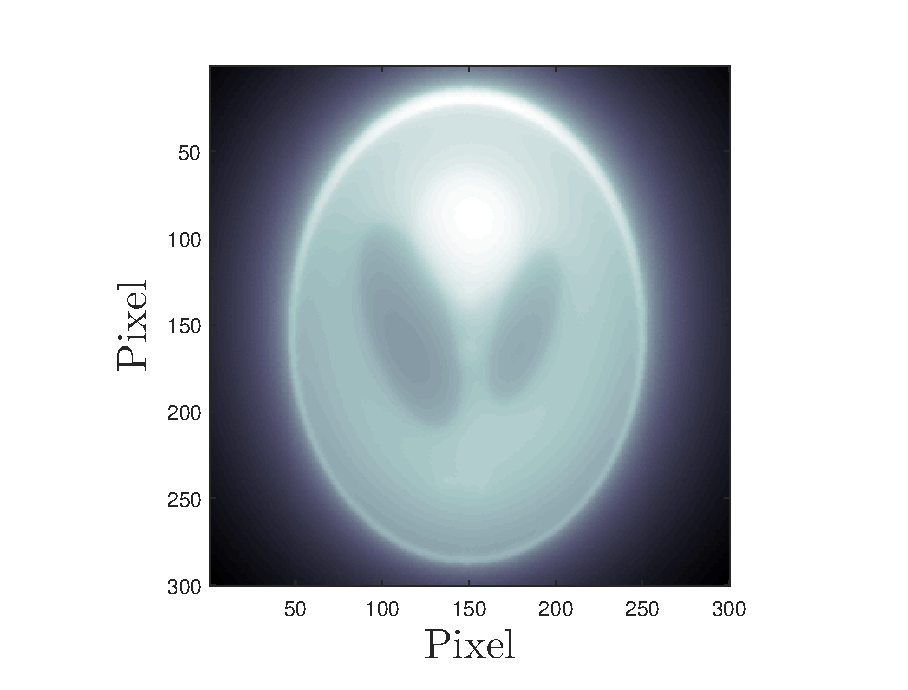
\includegraphics[width=0.5\textwidth]{backProjection.eps} }}
	\end{center}
	\caption{ Links (a) ist die Radontransformierte wie in der Abb. \ref{fig:3.2.b}. Rechts (b) ist die ungefilterte Rückprojektion von (b).}
	\label{fig:3.3}
\end{figure}

Jetzt wollen wir nachvollziehen, warum der Effekt der Verschwommenheit bei der ungefilterten Rückprojektion auftritt. Dazu sei zunächst die Abbildung \ref{fig:3.4} betrachtet, denn mit ihrer Hilfe können wir den Zusammenhang zweier Punkte in der Ebene $\Omega$ nachvollziehen.
\begin{figure}[H]
	\begin{minipage}[t]{0.4\textwidth}
		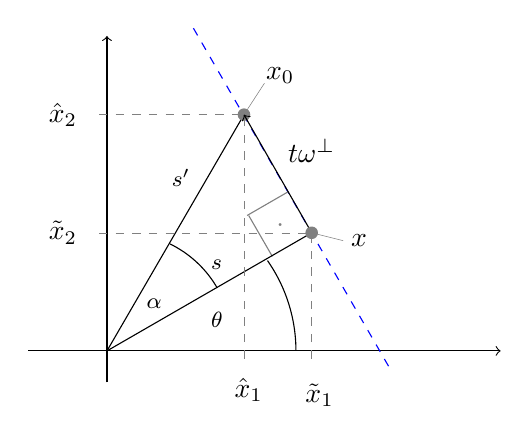
\begin{tikzpicture}[scale=2]		
			\draw [black] [->](-0.5,0) -- (2.5,0); % x-Achse
			\draw [black] [->](0,-0.2) -- (0,2); % y-Achse
			
			\draw [rotate=30, xshift=1.5cm, dashed] [blue] (0,1.5) -- (0,-1); % strahl
			
			\draw [xshift=1.05cm, yshift=0.6cm, rotate=120, - ] [gray] (0,0) -- (0.3,0);
			\draw [xshift=0.89cm, yshift=0.86cm, rotate=30, - ] [gray] (0,0) -- (0.3,0);
			\draw [gray] (1.1, 0.8)  node {$.$};
			
			\draw [black] [-] (0,0) -- (1.3,0.75); % s line
			\draw [black] (0.35, 1.1) node [right] {\footnotesize$s'$}; % s'
			\draw [dashed, very thin] [gray] (0.87,-0.05) -- (0.87,1.5); % \hat{x1} Projektion
			\draw [black] (0.9,-0.25)  node {$\hat{x}_1$};
			
			\draw [black] [-] (0,0) -- (0.87,1.5); % s' line
			\draw [black] (0.6, 0.55) node [right] {\footnotesize$s$}; % s
			\draw [dashed, very thin] [gray] (-0.05,1.5) -- (0.87,1.5); % \hat{x2} Projektion
			\draw [black] (-0.28,1.5)  node {$\hat{x}_2$};
			
			\fill[gray](0.87,1.5) circle [radius=0.04]; %x point 
			\draw[gray, very thin](0.87,1.5) -- (1, 1.7);
			\draw [black] (1.1, 1.75) node {$x_0$};
			
			\draw [black] [->] (1.3,0.75) -- (0.87,1.5); % t line
			\draw [black] (1.3,1.27) node {$t\omega^{\perp}$};	
			
			\fill[gray](1.3,0.75) circle [radius=0.04];
			\draw[gray, very thin](1.3,0.75) -- (1.5, 0.7);
			\draw [black] (1.6, 0.7) node {$x$};
			
			\draw [dashed, very thin] [gray] (1.3,-0.05) -- (1.3,0.75); % x-Projektion
			\draw [black] (1.35,-0.28)  node {$\tilde{x}_1$}; %\tilde{x1}
			
			\draw [dashed, very thin] [gray] (-0.05,0.75) -- (1.3,0.75); % y-Projektion		
			\draw [black] (-0.28,0.75)  node {$\tilde{x}_2$}; % \tilde{x2}
			
			\draw [black] (1.2,0) arc [start angle=0, end angle=35, radius=1cm]; % angle \theta
			\draw [black] (0.6, 0.2) node [right] {\footnotesize$\theta$};
			
			\draw [black] (0.7,0.4) arc [start angle=30, end angle=64, radius=0.7cm];
			\draw [black] (0.3, 0.3) node {\footnotesize$\alpha$};
		
		\end{tikzpicture}		
	\end{minipage}
	\begin{minipage}[b][5cm][t]{0.6\textwidth}
		\begin{align}
			& \beta = \alpha + \theta \label{equa:3.4}\\
			& x = \left(\begin{array}{c} \tilde{x_1} \\ \tilde{x_2} \end{array}\right) = s \left(\begin{array}{c} \cos(\theta) \\ \sin(\theta) \end{array}\right) = s\omega(\theta) \label{equa:3.5}\\
			& x_0 = \left(\begin{array}{c} \hat{x_1} \\ \hat{x_2} \end{array}\right) = s' \left(\begin{array}{c} \cos(\beta) \\ \sin(\beta) \end{array}\right) = s'\omega(\beta) \label{equa:3.6}\\
			& s'\omega(\beta) = s\omega(\theta) + t\omega^{\perp}(\theta)
			\label{equa:3.7}
		\end{align}
	\end{minipage}
	\caption{Eine Skizze (links) zur Verdeutlichung der Beziehung zweier Punkte $x_, x_0 \in \Omega$ bezüglich ihrer kartesischen- und Polar-Koordinaten. Die dazugehörige Nebenrechnung (rechts) zeigt deren formelmäßigen Zusammenhang auf.}
	\label{fig:3.4}
\end{figure}

Hier ist das Ziel zu zeigen dass, dass die ungefilterte Rückprojektion eine Faltung von $f(x) , \ x \in \Omega$ mit einer noch näher zu bestimmenden Funktion $h(x), \ x \in \Omega$ darstellt. Dazu formulieren wir folgendes Lemma:
\begin{lemma}
	Sei $f(x) \in L^2(\Omega)$ beliebig und $h(x) \in L^2(\Omega)$ speziell, dann kann die ungefilterte Rückprojektion als Faltung zweier Funktionen als
	\[ \mathcal{R^*} g(x_0) = \int \limits_{\R^2} f(x)h(x-x_0) \mbox{d}x = f(x)*h(x).\]	
	geschrieben werden. Da $\mbox{supp}f \subset \Omega$ betrachten wir das obige Integral nur auf $\Omega$.
	\label{lemma:3}
\end{lemma}
\begin{Bemerkung}
	Bevor wir zum Beweis übergehen, führen wir die dafür benötigte $\delta$-Distribution und einige für uns nützliche Eigenschaften ein. Seien $x, x_0 \in \R^2$, dann gilt:
	\begin{align}
	   	&  \ \  \delta(x-x_0) = \left\{ \begin{matrix} 0 & : &  x \neq x_0 \\ \infty & : & x = x_0 \end{matrix}\right. \label{equa:3.8}
   	\end{align}
	Eigenschaften :
	\begin{align}
		(\lowroman{1}).  &  \ \ \langle \delta(x-x_0), f(x)\rangle = \int \limits_{-\infty}^{\infty} f(x)\delta(x-x_0)\mbox{d}x = f(x_0) \label{equa:3.9}\\
		(\lowroman{2}). &  \ \  \delta(ax) = \frac{1}{|a|}\delta(x) \label{equa:3.10} \\
		(\lowroman{3}). &  \ \  \int \limits_{-\infty}^{-\infty}\delta(x-x_0) \mbox{d}x = 1 \label{equa:3.11}
	\end{align}
	\label{bem:8}
\end{Bemerkung}
\begin{proof}
	Wir Beginen mit der Definition der ungefilterten Rückprojektion (\ref{equa:1.21}) und benutzen dabei die Nebenrechnung zu Abb. \ref{fig:3.4} sowie die eingeführten Eigenschaften der $\delta$-Distribution aus der Bemerkung \ref{bem:8}.
	\begin{equation}
	\begin{split}
		\mathcal{R^*} g(x_0) & = \int\limits_{0}^{\pi} \ g(x_{0}^{T}\omega(\theta),\theta) \ \mbox{d}\theta  \ \  \stackrel{(\ref{equa:1.10}, \ \ref{equa:3.7})}{=} \ \ \int\limits_{0}^{\pi} \left( \int\limits_{-\gamma(s)}^{\gamma(s)} f(s'\omega(\beta)) \ \mbox{d}t \right) \mbox{d}\theta \\
		& \stackrel{(\ref{equa:3.9})}{=} \int\limits_{0}^{\pi} \left( \int\limits_{-\gamma(s)}^{\gamma(s)} \int\limits_{-1}^{1} f(s\omega(\theta)) \delta(s\omega(\theta) - s'\omega(\beta)) \ \mbox{d}s \ \mbox{d}t \right) \mbox{d}\theta \\
		& \stackrel{(\ref{equa:3.7})}{=} \int\limits_{0}^{\pi} \left( \int\limits_{\Omega} f(x) \delta(t\omega^{\perp}(\theta)) \ \mbox{d}x \right) \mbox{d}\theta \stackrel{(\ref{equa:3.10})}{=} \int\limits_{\Omega} f(x) \frac{\int\limits_{0}^{\pi}\delta(\beta - \alpha)\mbox{d}\beta}{|t\frac{\partial \omega^{\perp}(\theta)}{\partial \theta}|} \mbox{d}x \\
		& \stackrel{(\ref{equa:3.11})}{=} \int\limits_{\Omega} f(x) \frac{1}{|x - x_0|} \mbox{d}x = f(x)*h(x).
	\end{split}
	\label{equa:3.12}
	\end{equation}
	In der letzten Zeile wurde $|t\frac{\partial \omega^{\perp}(\theta)}{\partial \theta}| = |t||\left(\begin{array}{c} -\cos(\theta) \\ -\sin(\theta) \end{array}\right)| = |t| = |x -x_0|$ benutzt.
\end{proof}
Somit haben wir auch die spezielle Funktion $h(x) = \frac{1}{|x|}$ gefunden. Die Funktion $h$ heißt \textit{Point-Spread-Function}. Anschaulich kann $f$ in jedem Punkt als $\delta$-Distribution verstanden werden. Das heißt, setzt man $f$ auf ganz $\Omega$ Null, außer im Punkt $x_0 \in \Omega$ und faltet mit $h(x)$, so wird das Ergebnis $\tilde{f}$ um den Punkt $x_0$ nach außen radial abfallen. Führt man die Faltung von $f$ für jeden Punkt in $\Omega$ und setzt auf diese Weise entstandene Faltungsbilder zusammen führt das zu dem Effekt der Verschwommenheit. 

\subsection*{Gefilterte Rückprojektion}
\label{cha:3.1.2}

Das in dem letzten Abschnitt erreichte Ergebnis ist für die Praxis unbrauchbar. Man kann an einem verschwommenen Bild keine qualitative Analyse durchführen. Deshalb werden wir in diesem Abschnitt eine Verbesserung des ersten Verfahrens suchen. Wie der Name schon verrät, bekommt man ein ungefiltertes Bild zurück. Wir wollen nun verstehen, wie man die Projektionsdaten filtert, bevor man sie zurück projiziert.

Um den Ausdruck der \textit{gefilterten Rückprojektion} zu bekommen, werden wir uns des sogenannten \textit{Fourier\footnote{Jean Baptiste Joseph Fourier (1768 - 1830) ein französischer Mathematiker und Physiker.}-Slice-Theorem} (FST) bedienen (siehe z.B. \cite[S. 120]{Buzug04}). Das Schema des Theorems kann nun folgendermaßen wiedergegeben werden:
\begin{enumerate}
	\item Berechne für einen festen Winkel $\theta$ die Fouriertransformierte\footnote{
		\label{foot:14}\textbf{Definition }\textit{Fourier-Transformation}. Sei $f(x) \in L^2(\Omega)$, dann ist ihre Fourier-Transformation durch
			\begin{equation}
				(\mathcal{F}f)(x) = \int \limits_{\Omega} f(x) e^{-2\pi i \langle x^T, u \rangle} \mbox{d}x = F(u), \ \ u \in \mathbb{C}^2
				\label{equa:3.13}
			\end{equation}
		gegeben.} (FT) einer Projektion $\mathcal{R}f(s,\theta) = g(s,\theta)$
	\[(\mathcal{F}g)(s,\theta) = G(q, \theta). \]
	\item Konstruiere die Fouriertransformierte $F(u,v)$ von $f(x)$ aus $G(q,\theta)$
	\[G(q,\theta) \leadsto F(u).\]
	\item Berechne die inverse Fouriertransformierte von $F$
	\[(\mathcal{F}^{-1}F)(u) = \tilde{f}(x). \]
\end{enumerate}

Wir werden den Punkt 2 des FST vom Punkt 1 und dann vom Punkt 3 aus schrittweise annähern. Bevor wir die Herleitung der gefilterten Rückprojektion angehen, machen wir uns die vorliegende Situation an einer Skizze (Abb. \ref{fig:3.5}) klar. 

In der Abbildung \ref{fig:3.5} ist schematisch wiedergegeben, dass die Fourier-Transformation an der Natur der Koordinatensysteme nichts ändert. Diese Tatsache wird in dem \textit{Plancherel-Theorem} bewiesen, welches unter anderem besagt, dass die die FT ein \text{unitärer} Operator für Funktionen aus $L^2$ ist. Das heißt, die FT ist linear, isometrisch und bijektiv. Das weiteren beweist der Satz die Invertierbarkeit von $\mathcal{F}$ für $L^2$ Funktionen. 
\begin{figure}[!h]
	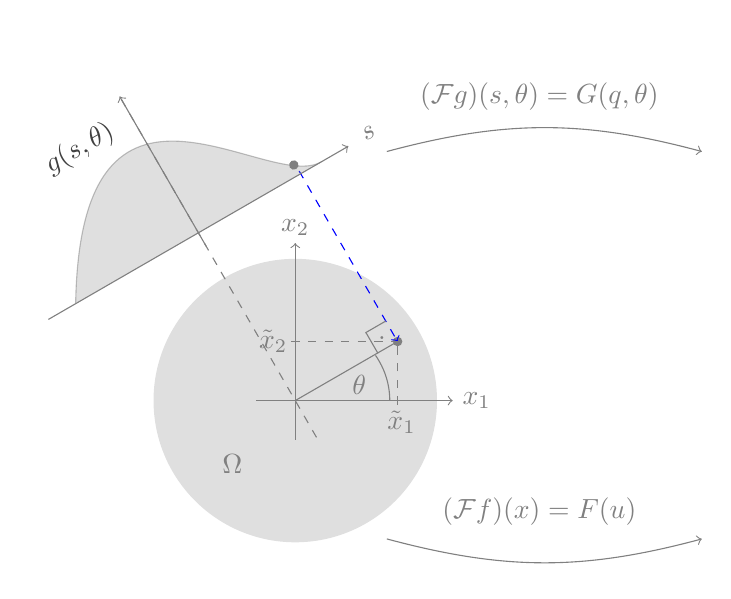
\begin{tikzpicture}[xshift=-100]%, scale=0.75]
		\fill[nearly transparent, color=gray] (0,0) circle (1.8cm);
		\draw [gray] [->](-0.5,0) -- (2,0); % x-Achse
		\draw [gray] (2, 0) node [right] {$x_1$};
		
		\draw [gray] [->](0,-0.5) -- (0,2); % y-Achse
		\draw [gray] (0, 2.2) node {$x_2$};
	
		\fill[gray](1.3,0.75) circle [radius=0.06]; % ein Punkt		
	
		\draw [rotate=30, xshift=1.5cm, ->, dashed] [blue] (0,2.5) -- (0,0); % strahl		
		
		\draw [xshift=1.05cm, yshift=0.6cm, rotate=120, - ] [gray] (0,0) -- (0.3,0);
		\draw [xshift=0.89cm, yshift=0.86cm, rotate=30, - ] [gray] (0,0) -- (0.3,0);
		\draw [gray] (1.1, 0.8)  node {$.$};
		
		\draw [rotate=30] [gray] [-] (0,0) -- (1.5, 0);
		
		\draw [dashed] [gray] (1.3,-0.05) -- (1.3,0.75); % x-Projektion
		\draw [gray] (1.35,-0.28)  node {$\tilde{x}_1$};
		
		\draw [dashed] [gray] (-0.05,0.75) -- (1.3,0.75); % y-Projektion		
		\draw [gray] (-0.28,0.75)  node {$\tilde{x}_2$};
		
		\draw [lightgray] [rotate=30, yshift=70] (-1.8,0) .. controls (0,3) and (1,0) .. (1.8,0);
		\fill [nearly transparent, color=gray] [rotate=30, yshift=70] (-1.8,0) .. controls (0,3) and (1,0) .. (1.8,0);
		
		\fill[ rotate=30, xshift=0.18cm, yshift=1.85cm, gray](1.3,0.75) circle [radius=0.06]; % ein Punkt
		
		\draw [rotate=30, xshift=0, yshift=70] [gray] [->] (-2.2,0) -- (2.2, 0); % s line
		\draw [gray] (3.7, 0)  node [rotate=30, xshift=-20, yshift=123] {$s$};
		
		\draw [rotate=120, xshift=70 ] [gray] [->] (-0.2,0) -- (2, 0);	% g(s, \theta) line	
		\draw [rotate=120, xshift=70 ] [gray, dashed] [-] (-3,0) -- (2, 0);		
		\draw [darkgray] (-0.2, 0)  node [left, rotate=30, yshift=115] {$g(s, \theta)$};		
		
		\draw [gray] (1.2,0) arc [start angle=0, end angle=35, radius=1cm];
		\draw [gray] (0.6, 0.2) node [right] {$\theta$};
		
		\draw [gray] (-0.8, -0.8) node {$\Omega$};
		
		\draw [gray] (3.1, 0) [rotate=0, xshift=0, yshift=110] node {$(\mathcal{F}g)(s,\theta) = G(q, \theta)$};
		\draw[->, gray] [rotate=0, xshift=90, yshift=90] (-2,0) to[out=15, in=165] (2,0);
		
		\draw [gray] (3.1, 0) [rotate=0, xshift=0, yshift=-40] node {$(\mathcal{F}f)(x) = F(u)$};
		\draw[->, gray] [rotate=0, xshift=90, yshift=-50] (-2,0) to[out=-15, in=195] (2,0);	
	\end{tikzpicture}
	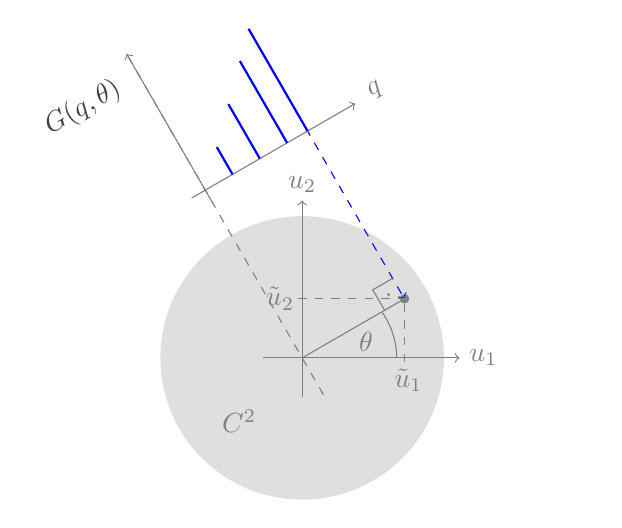
\begin{tikzpicture}[xshift=50]	
		\fill[nearly transparent, color=gray] (0,0) circle (1.8cm);
		\draw [gray] [->](-0.5,0) -- (2,0); % x-Achse
		\draw [gray] (2, 0) node [right] {$u_1$};
		
		\draw [gray] [->](0,-0.5) -- (0,2); % y-Achse
		\draw [gray] (0, 2.2) node {$u_2$};
		
		\fill[gray](1.3,0.75) circle [radius=0.06]; % ein Punkt		
		
		\draw [rotate=30, xshift=1.5cm, ->, dashed] [blue] (0,2.5) -- (0,0); % strahl		
		
		\draw [xshift=1.05cm, yshift=0.6cm, rotate=120, - ] [gray] (0,0) -- (0.3,0);
		\draw [xshift=0.89cm, yshift=0.86cm, rotate=30, - ] [gray] (0,0) -- (0.3,0);
		\draw [gray] (1.1, 0.8)  node {$.$};
		
		\draw [rotate=30] [gray] [-] (0,0) -- (1.5, 0);
		
		\draw [dashed] [gray] (1.3,-0.05) -- (1.3,0.75); % x-Projektion
		\draw [gray] (1.35,-0.28)  node {$\tilde{u}_1$};
		
		\draw [dashed] [gray] (-0.05,0.75) -- (1.3,0.75); % y-Projektion		
		\draw [gray] (-0.28,0.75)  node {$\tilde{u}_2$};
	
		\draw [rotate=30, xshift=0, yshift=70] [gray] [->] (-0.2,0) -- (2.2, 0);
		\draw [gray] (3.7, 0)  node [rotate=30, xshift=-20, yshift=123] {$q$};
		
		\draw [rotate=120, xshift=70 ] [gray] [->] (-0.2,0) -- (2, 0);	% g(s, \theta) line	
		\draw [rotate=120, xshift=70 ] [gray, dashed] [-] (-3,0) -- (2, 0);		
		\draw [darkgray] (-0.2, 0)  node [left, rotate=30, yshift=115] {$G(q, \theta)$};			
		
		\draw [gray] (1.2,0) arc [start angle=0, end angle=35, radius=1cm];
		\draw [gray] (0.6, 0.2) node [right] {$\theta$};
		
		\draw [gray] (-0.8, -0.8) node {$\mathbb{C}^2$};
		
		\foreach \x in {0, 0.4, 0.8, 1.2, 1.5}
		{
			\draw[rotate=30, xshift=0, yshift=70][blue, thick] (\x,\x) -- (\x,0); 
		}
	\end{tikzpicture}
	\caption{Eine Veranschaulichung des Fourier-Slice-Theorems. Links ist der Vorgang der Radon Transformation abgebildet, rechts seine Fouriertransformierte.}
	\label{fig:3.5}
\end{figure}

Jetzt haben wir genug Argumente gesammelt, um die gefilterte Rückprojektion herzuleiten. Dafür beginnen wir mit dem Punkt 1 des FST: wir bilden die Fouriertransformierte (Fußnote \ref{foot:14}) einer Projektion $p(s, \theta)$:
\begin{equation}
	\begin{split}
		P(q, \theta) & = \int \limits_{-1}^{1} p(s, \theta) e^{-2\pi i qs} \mbox{d}s \\
		&  \stackrel{(\ref{equa:1.10})}{=} \int \limits_{-1}^{1} \left( \int\limits_{-\gamma(s)}^{\gamma(s)} f(s\omega(\theta) + t\omega^{\perp}(\theta)) \mbox{d}t \right) e^{-2\pi i qs} \mbox{d}s \\
		& \stackrel{(\ref{equa:1.22})}{=} \int \limits_{\Omega} f(x) e^{-2\pi i q x^T\omega(\theta)}\mbox{d}x.	
	\end{split}
	\label{equa:3.14}
\end{equation}	
An dem Punkt 3 des FST ist nicht viel zu tun, deshalb geben wir hier direkt die Fouriertransformierte von $f$ an. Bei der Wahl der Koordinaten für $\mathcal{F}f$ und ihre Umrechnung stützen wir uns auf die rechte Seite der Abbildung \ref{fig:3.5}. Dann gilt 
\begin{equation}
	 F(q\cos(\theta), q\sin(\theta)) = \int \limits_{\Omega}^{} f(x)e^{-2\pi i qx^T\omega(\theta)} \mbox{d}x.
	\label{equa:3.15}
\end{equation}
Aus den Gleichungen (\ref{equa:3.14}) und (\ref{equa:3.15}) können wir festhalten, dass die Fouriertransformierten von $f$ und $p$ im folgenden Bezug zueinander stehen
\begin{equation}
	F(q\cos(\theta), q\sin(\theta)) =  P(q, \theta).
	\label{equa:3.16}
\end{equation}   
Das heißt (\ref{equa:3.16}) soll eine Koordinatentransformation zwischen $\mathcal{F}f$ und $\mathcal{F}p$ darstellen. Somit ist der Punkt 2 des FST auch erledigt.

Im zweiten Schritt invertieren wir die Gleichung (\ref{equa:3.15}) und führen eine Variablensubstitution\footnote{Für die Substitution von $\mbox{d}u_1\mbox{d}u_2$ berechnen wir die Jacobi-Determinante von $ |J(\left(\begin{array}{c} u_1 \\ u_2 \end{array}\right)) = \left| \left(\begin{pmatrix}{c} \cos(\theta) & \sin(\theta) \\ -q\sin(\theta) & q\cos(\theta) \end{pmatrix}\right)\right| = q$, somit erhalten wir $\mbox{d}u_1\mbox{d}u_2 = q\mbox{d}q\mbox{d}\theta$.} durch, sodass man zu der Gleichung  
\begin{equation}
	f(x) = \int \limits_{0}^{\pi} \int \limits_{-1}^{1}F(q\cos(\theta), q\sin(\theta))e^{2\pi i qx^T\omega(\theta)} q \ \mbox{d}q \ \mbox{d}\theta
	\label{equa:3.17}
\end{equation}
gelangt. Die Symmetriebetrachtungen, wie in \cite[S. 135]{Buzug04} und die Tatsache, dass man nur reelle Funktionen auf $\Omega$ betrachtet, führen zu folgendem Ausdruck
\begin{equation}
	\begin{split}
		f(x) & = \int \limits_{0}^{\pi} \int \limits_{-1}^{1}F(q\cos(\theta), q\sin(\theta))e^{2\pi i qx^T\omega(\theta)} |q| \ \mbox{d}q \ \mbox{d}\theta \\
		& \stackrel{(\ref{equa:3.16})}{=} \int \limits_{0}^{\pi} \left( \int \limits_{-1}^{1} \left( \ P(q, \theta)|q| \ \right) e^{2\pi i qx^T\omega(\theta)} \ \mbox{d}q \right) \mbox{d}\theta.
	\end{split}
	\label{equa:3.18}
\end{equation}

Mit der Gleichung (\ref{equa:3.18}) haben wir die gefilterte Rückprojektion erhalten. Es bleibt noch das Gefilterte darin zu entdecken. Beginnen wir mit der inneren Klammerung von (\ref{equa:3.18}). $P(q, \theta)$ ist die Fouriertransformierte $\mathcal{F}p$ von $p(s,\theta)$, die punktweise mit einer Betragsfunktion $b(q) = |q|$ multipliziert wird. Da wir jetzt $p(s, \theta)$ im Frequenzraum betrachten und die Funktion $b(q)$ über das gleiche Frequenzband, wie $P(q,\theta)$ läuft, werden durch punktweise Multiplikation kleinfrequente Anteile von $P(q,\theta)$ von $b(q)$ unterdrückt und die hochfrequente im Gegensatz sehr verstärkt. Dieses Vorgehen wird im Allgemeinen \textit{Hochpassfilterung} genannt. Die Funktion $b(q) = |q|$ bezeichnet man als Rampenfilter. Im Folgenden bezeichnen wir einen Filter mit $h_{\xi}(q)$ und wir schreiben $h_{b}(q) = b(q) = |q|$. Für die Filterung der Projektionen führen wir die Bezeichnung $P_{h_{\xi}}(q, \theta) = P(q, \theta)h_{\xi}(q)$ ein.

Nach dem die Filterung der Projektion durchgeführt wurde, wird diese mittels der inversen FT zurück in den Ortsrum der Projektionen überführt. Was durch das innere Integral von (\ref{equa:3.18}) dargestellt wird. Anschließend projiziert man die gefilterte Projektion in den Ortsraum von $f$ zurück, dies ist das äußere Integral von (\ref{equa:3.18}). 

Wir fassen die nötigen Schritte der gefilterten Rückprojektion zu einem Algorithmus zusammen
\begin{algorithm}
	\caption{Gefilterte Rückprojektion (Filtered Back Projection, FBP)}
	\begin{algorithmic}[1]	
		\State Berechne die FT von $(\mathcal{F}p)(s, \theta) = P(s, \theta)$.
		\State Führe die Fiterung $P_{h_{\xi}}(q, \theta) = P(q, \theta)h_{\xi}(q)$ durch.
		\State Berechne die inverse FT $(\mathcal{F}^{-1}P_{h_{\xi}})(q, \theta) = \tilde{p}(s,\theta)$.
		\State Projiziere $\tilde{p}(s,\theta)$ auf $\Omega$ zurück. 
	\end{algorithmic}
	\label{alg:3.1}
\end{algorithm}

In der Abbildung \ref{fig:3.6.b} ist das erste Ergebnis der gefilterten Rückprojektion, gefiltert mit einem Rampenfilter zu sehen. 

Wenn man das Sinogramm (Abb. \ref{fig:3.2.b}) betrachtet, so stellt man fest, dass das Sinogramm keine Störungen aufweist. Das würde eine perfekte Messung bedeuten. Dies ist aber bei den realen Messungen nie der Fall. Deshalb wollen wir uns die Rekonstruktion von gestörten Daten anschauen. Dafür soll das Phantom Bild (Abb. \ref{fig:3.2.a}) mit einem Salzstreuer-Effekt (Quelle: \MATLAB) beaufschlagt werden. Das soll die Homogenität einiger Pixelbereiche von der Abbildung \ref{fig:3.2.a} aufheben, was eine kleine Annäherung zur Realität widerspiegelt (Abb. \ref{fig:3.7.a}).  
\begin{figure}[!h]
	\begin{center}
		\subfloat[\label{fig:3.6.a}Das Rampenfilter.]{{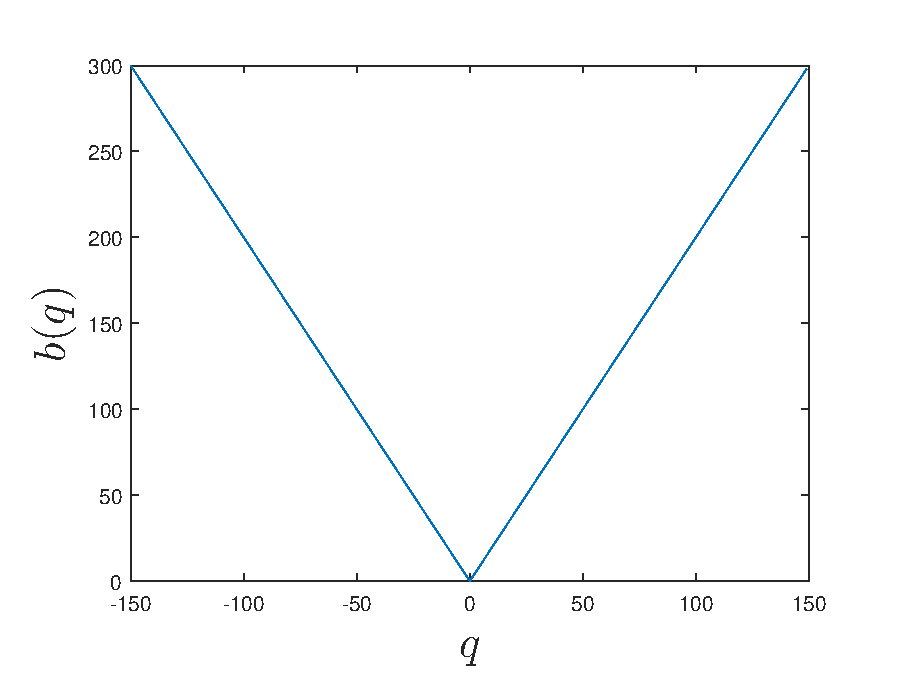
\includegraphics[width=0.5\textwidth]{rampFilter.eps} }}
		\subfloat[\label{fig:3.6.b}Eine mit Rampenfilter gefilterte Rückprojektion.]{{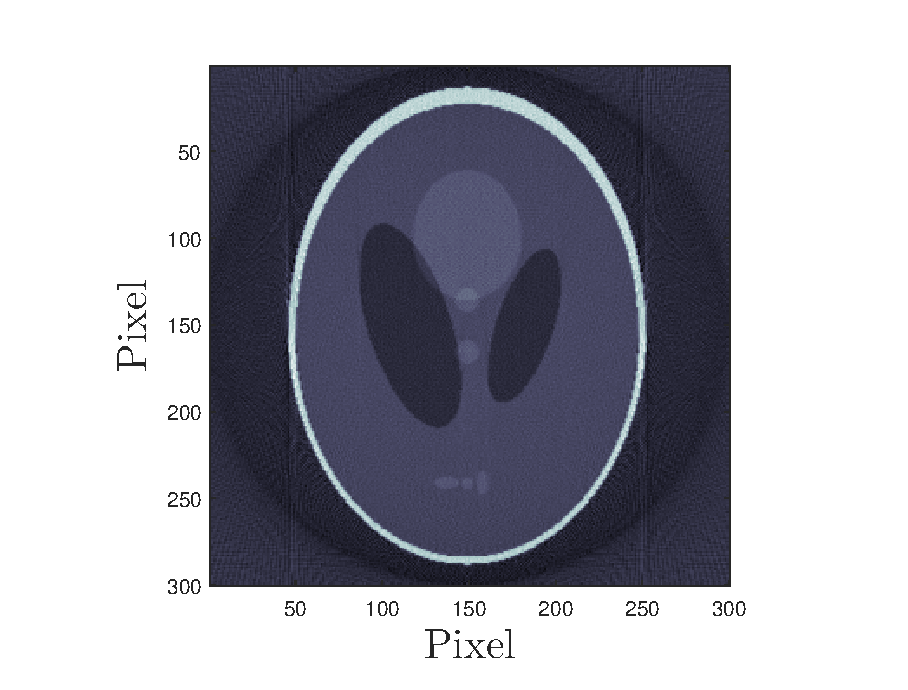
\includegraphics[width=0.5\textwidth]{rampFiltered.eps} }}
	\end{center}
	\caption{ Links (a) das Rampenfilter, konstruiert passend zu dem Sinogramm aus \ref{fig:3.2.b}. Das Frequenzband des Filters ist durch die isometrische Eigenschaften der FT gleich der Detektorbreite, also ist auch gleich der Tiefe des Sinogramms. Rechts (b) ist die gefilterte Rückprojektion von \ref{fig:3.2.b}, durchgeführt unter der Einwirkung des Rampenfilters aus (a).}
	\label{fig:3.6}
\end{figure} 

Die Radon Transformation von der Abbildung \ref{fig:3.7.a} ohne zusätzliche Störung würde nicht die Messfehler repräsentieren, höchstens Rundungsfehler, die bei der Integration entstehen, hier aber nicht wesentlich sind. Deshalb stören wir die Projektionsdaten zusätzlich mit dem Salzstreuer-Effekt (Abb. \ref{fig:3.7.b}).
\begin{figure}[!h]
	\begin{center}
		\subfloat[\label{fig:3.7.a}Ein verrauschtes Phantombild.]{{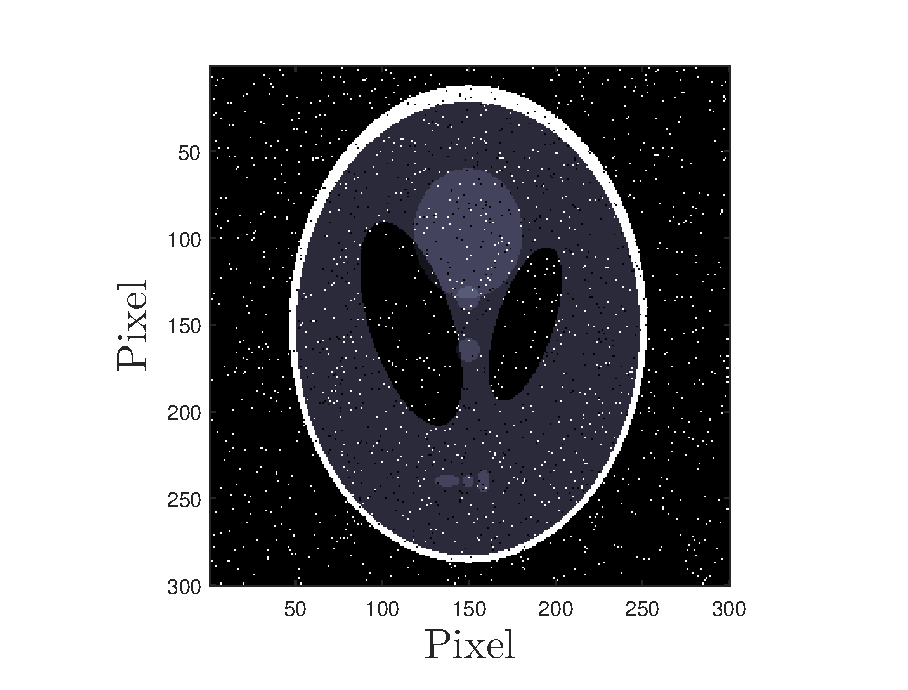
\includegraphics[width=0.5\textwidth]{noisedPhantom.eps} }}
		\subfloat[\label{fig:3.7.b}Die Radontransformierte von (a) und einem zusätzlichem Rauschen.]{{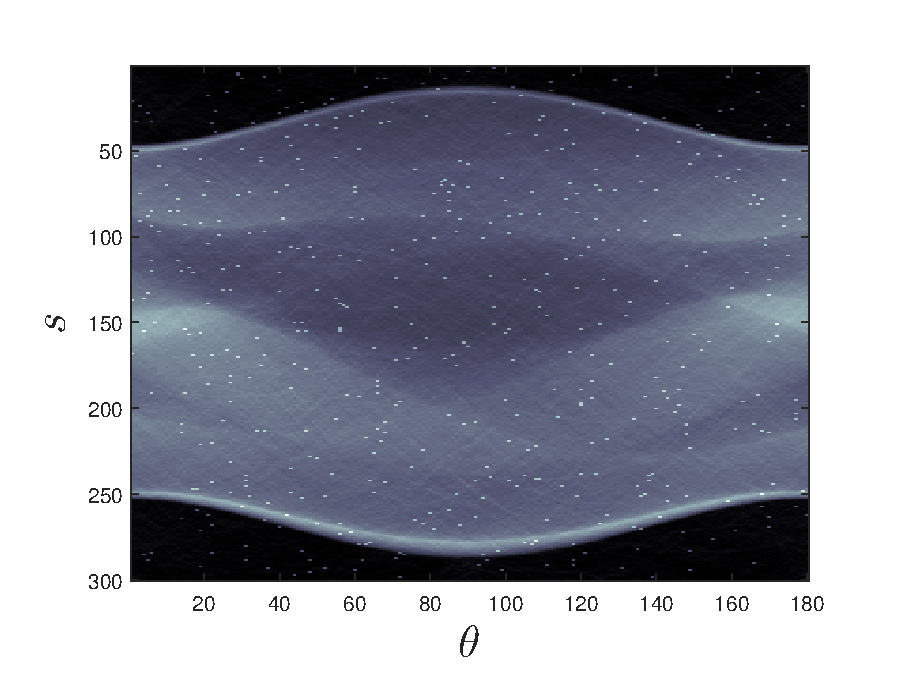
\includegraphics[width=0.5\textwidth]{rt_noised.eps} }}
	\end{center}
	\caption{ Links (a) ist ein Phantombild verrauscht mit einem Salzstreuer-Effekt (Quelle: \MATLAB) dargestellt. Rechts (b) ist Die Radontransformierte von (a) und zusätzlich mit einem Salzstreuer-Effekt verrauscht.}
	\label{fig:3.7}
\end{figure} 

Wir erinnern uns an die Ergebnisse des zweiten Kapitels. Insbesondere daran, dass der Operator $\mathcal{R}$ schlecht gestellt ist. Dazu sei die Gleichung (\ref{equa:2.3}) nochmal betrachtet
\[\mathcal{R}^{+} g  = \sum\limits_{j = 1}^{n} \sigma_j^{-1} \langle g, u_j \rangle_{L^2(Z)} v_j.\]
Wir wissen, dass $g$ die Projektionen in (\ref{equa:2.3}) darstellt. Sei nun $p_{\epsilon}$ unsere gestörte Projektion. Des Weiteren betrachten wir den Schritt 2,3 des Algorithmus \ref{alg:3.1} und schreiben ihn, wie folgt auf
\begin{eqnarray}
	\tilde{p}_{\epsilon} = \int \limits_{-1}^{1} P(q, \theta)h_{\xi}(q) e^{2\pi i qx^T\omega(\theta)} \ \mbox{d}q.
	\label{equa:3.19}
\end{eqnarray}
Wir wollen nun $\tilde{p}_{\epsilon}$ als eine Linearkombination oder auch als verallgemeinerte Fourierreihe angeben. Das tun wir direkt für den diskreten Fall unter Beachtung der Bemerkung \ref{bem:5}. Somit bekommen wir
\begin{equation}
	\tilde{p}_{\epsilon} \approx \sum \limits_{i = 1}^{n} c_ih_{\xi}(q_i)u_i, \ \ \mbox{mit} \  c_i = \langle \tilde{P}, u_i \rangle.
	\label{equa:3.20}
\end{equation} 
Diese Gleichung werden wir nicht beweisen, aber praktisch bedeutet das, wenn man $h_{\xi}(q) = 1$ setzt und es dem FBP Algorithmus übergibt, kommt genau die ungefilterte Projektion dabei raus.
\begin{figure}[!h]
	\centering
	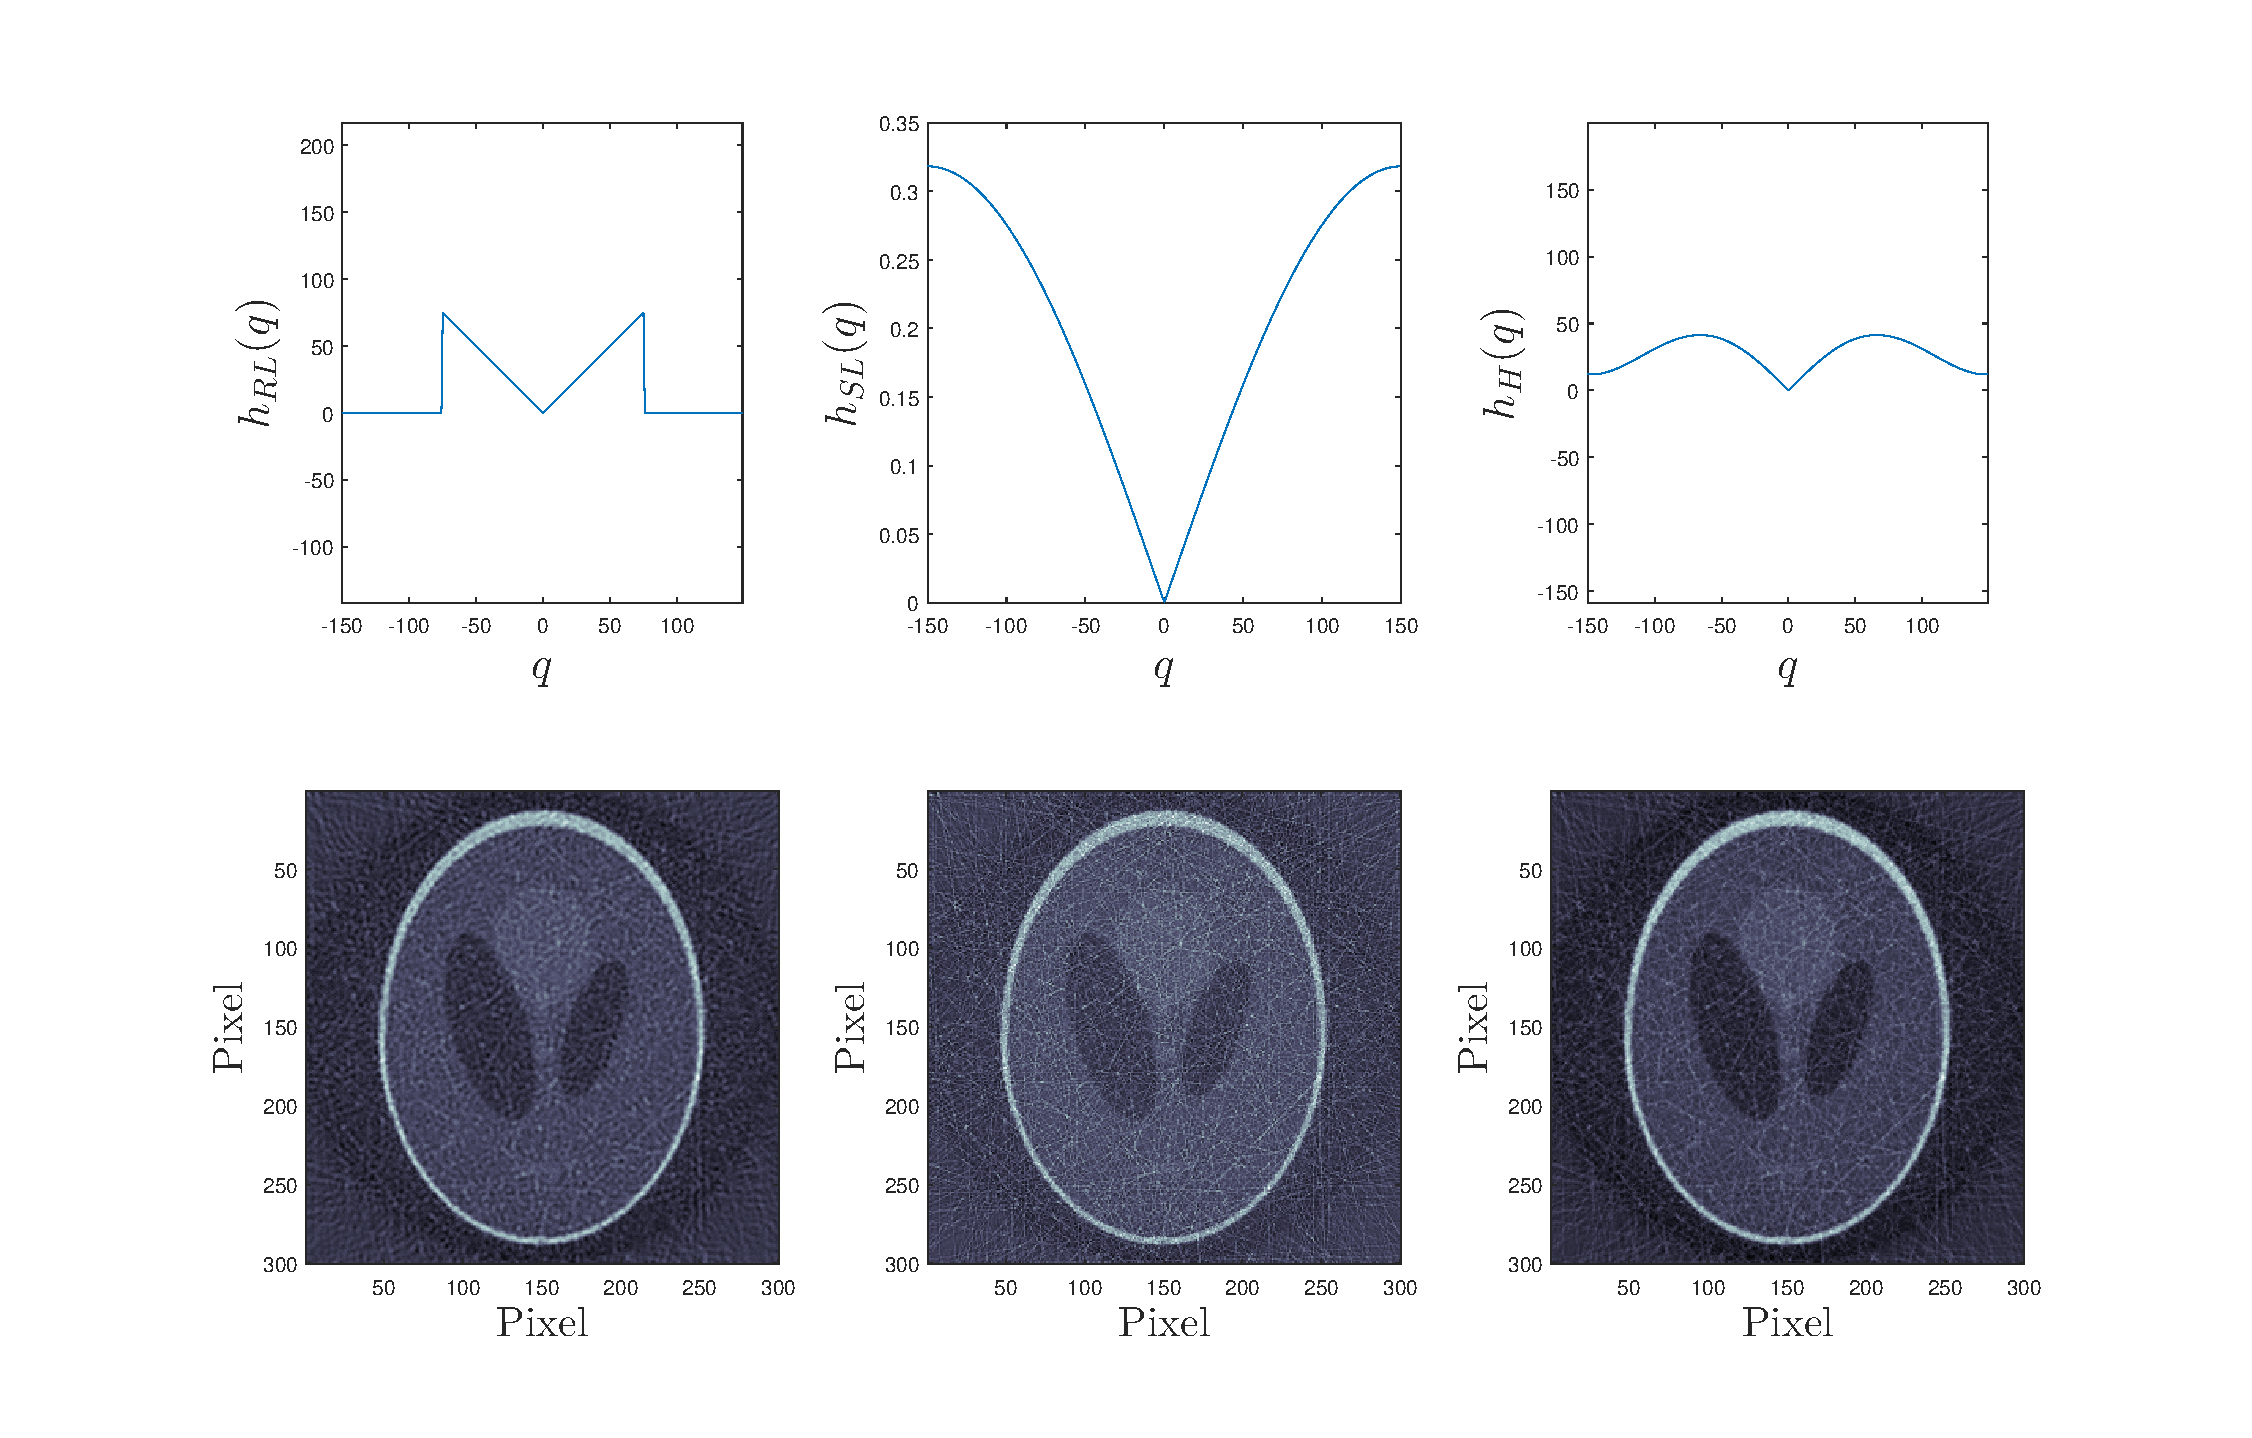
\includegraphics[width=1\textwidth]{diffFilter.eps}
	\caption{Eine Rekonstruktion aus den Daten \ref{fig:3.7.b} unter der Einwirkung von drei verschiedenen Filtern. Unten links ist die Filterung mit dem \textit{Ramachandran-Lakshminarayanan-Filter}, mittig mit dem \textit{Shepp-Logan-Filter} und rechts mit dem \textit{Hamming-Fiter} dargestellt.}  
	\label{fig:3.8}
\end{figure}

Nun setzen wir unsere gestört-gefilterte Projektion (\ref{equa:3.20}) in (\ref{equa:2.3}) ein und bekommen einen Ausdruck
\begin{equation}
	\begin{split}
		\mathcal{R}^{+} g & = \sum\limits_{j = 1}^{n} \sigma_j^{-1} \langle \left( \sum \limits_{i = 1}^{n} c_i h_{\xi}(q_i) u_i \right), u_j \rangle_{L^2(Z)} v_j \\
		& = \sum\limits_{j,i = 1}^{n} ( \sigma_j^{-1} h_{\xi}(q_j) ) c_i \delta_{ij} v_j = \sum\limits_{j = 1}^{n} ( \sigma_j^{-1} h_{\xi}(q_j) ) c_i v_j,
	\end{split}
	\label{equa:3.21}
\end{equation}
der uns prinzipiell keine neue Erkenntnis liefert, aber offensichtlich macht, wie die hochfrequenten Anteile bei der Rekonstruktion von dem Filter beeinflusst werden können. Das heißt, das Design des Filters kann die Rückprojektion in verschiedenen Frequenzbereichen dämpfen und somit ihre Oszillation bis zu einem gewissen Grade beschränken. Anders gesagt, wir beschleunigen somit die Konvergenz der Reihe (\ref{equa:3.21}) zu unseren Gunsten. 

In der Abbildung \ref{fig:3.8} sind drei Ergebnisse mit drei verschiedenen Filtern dargestellt. Zum Aufbau verschiedener Filterkerne sei man hier auf \cite[S. 191]{Buzug04} verwiesen. In der Abbildung \ref{fig:3.8} links unten, ist zu erkennen, dass ein \textit{Ramachandran-Lakshminarayanan-Filter} die hohen Frequenzen abschneidet, wodurch das Bild insgesamt an Kontrast verliert. Das untere Ergebnis in der Mitte zeigt, dass das \textit{Shepp-Logan-Filter} die mittleren Frequenzen anhebt, was die Helligkeit des Ergebnisses etwas erhöht. Das untere rechte Bild hat durch das \textit{Hamming-Fiter} volles Frequenzband erhalten, allerdings sind die hohen Frequenzen stark gedämpft worden.

Insgesamt existiert ein Dutzend Filter, die bei der CT-Bildrekonstruktion eingesetzt werden können. Dieses Vorgehen nennt man \textit{Regularisierung} des Rückprojektionsproblems mit Filtern.  

\section*{Algebraische Rekonstruktionsverfahren}
\label{cha:3.2}

Algebraische Verfahren basieren auf der Auffassung des Operators $\mathcal{R}$ als eine Matrix. Das hat zu Folge, dass man die Wirkung von $\mathcal{R}$ auf $f$ in Form eines linearen Gleichungssystems auffassen kann. Somit bekommen wir
\begin{equation}
	\mathcal{R}f = Af = p.
	\label{equa:3.22}
\end{equation}
\begin{Bemerkung}
	Für den Rest dieses Kapitels vereinbaren wir nur diskretisierte Systeme zu betrachten. 
	\label{bem:9}
\end{Bemerkung}
Mit der Bemerkung \ref{bem:9} und den vereinbarten Größen $f \in \R^m$ (\ref{equa:3.2}) und $p \in \R^n$ (\ref{equa:3.1}) ist $A$ eine endliche Matrix. $A$ wird \textit{Systemmatrix} des Abbildungssystems von $\mathcal{R}$ genannt. Wir werden zunächst die Entstehung und den Aufbau von $A$ etwas genauer anschauen. 

\subsubsection{Aufbau der Systemmatrix $A$ von $\mathcal{R}$}

Da $f \in \R^m$ und $p \in \R^n$ sind bedeutet es, dass $A \in \R^{n\times m}$ ist. Das heißt, die Zeilen von $A$ laufen über die Indizierung der Projektionen $p$, also die Zeile $j$ ist die $j$-te Projektion. Die Spalten von $A$ laufen über die Indizierung von $f$.

$f$ wird durch die Anzahl der Detektoren $k$ im Detektorband diskretisiert (Abb. \ref{fig:3.9}). Man kann also hypothetisch $f \in \R^{k\times k}$ annehmen. Lassen wir die Indizierung von $f$ Zeilenweise durchlaufen, so kommen wir genau auf $f \in \R^{k^2}$. Wobei nach (\ref{equa:3.2}) $k^2= m$ gilt.

Aus der Gleichung (\ref{equa:3.22}) können wir folgern, dass für $j$-te Projektion
\begin{equation}
	\sum \limits_{i = 1}^{m} a_{ji}f_i = p_j
	\label{equa:3:23}
\end{equation}
gelten muss. Beachtet man, dass nur die $f_j$ die vom Strahl getroffen worden sind zur Summe (\ref{equa:3:23}) beitragen, ergibt sich die Gleichung (\ref{equa:3.3}).
\begin{figure}[!h]
	\centering
	\begin{tikzpicture}
	\fill[nearly transparent, color=gray] (0,0) circle (2cm);
	\draw [gray] (-1, -1) node {$\Omega$};
	\draw [step=0.4,blue, thin, rotate=90, xshift=0, yshift=90] (-2,0) grid (2,0.4); % detector grid
	
	\draw [step=0.4, lightgray, very thin] (-2,-2) grid (2,2); % picture grid
	
	\draw [black] [->](-0.5,0) -- (2.5,0); % x-Achse
	\draw [black] (2.5, 0) node [right] {$x_1$};
	
	\draw [black] [->](0,-0.5) -- (0,2.4); % y-Achse
	\draw [black] (0, 2.6) node {$x_2$};
	
	\draw [rotate=90, xshift=0cm, <-, dashed] [blue] (1.4,3) -- (1.4,-2.2); % strahl
	%\draw [rotate=30, xshift=1.3cm ] [black] (0,-2.2) node {Röntgenstrahl};
	
	\draw [rotate=90, xshift=0, yshift=90] [black] [->] (-2.5,0) -- (2.5, 0);
	\draw [black] (2.8, 0)  node [rotate=90, xshift=2.7cm, yshift=6cm] {$s$};
	
	
	\draw [rotate=90, xshift=0cm, dashed] [nearly transparent, color=black] (0,-2.5) -- (0,3.9); % punktiert Mitte
	\draw [rotate=0, xshift=0cm, dashed] [nearly transparent, color=black] (0,-2.5) -- (0,3.9); % punktiert Mitte
	
	\draw [black] (0.7,0) arc [start angle=0, end angle=90, radius=0.7cm]; % angle \theta
	\draw [black] (0.25, 0.25) node {\footnotesize$\theta_l$};
	
	\draw [step=0.4, red, thin, rotate=90, xshift=1.2cm, yshift=0] (0,-2) grid (0.4,2);

	
	\draw [black] (0, 0)  node [rotate=0, xshift=1.4cm, yshift=-1.9cm] {\footnotesize$...$};
	\draw [black] (0, 0)  node [rotate=0, xshift=1.8cm, yshift=-1.8cm] {\footnotesize$f_{k^2}$};
		
	\draw [rotate=0, xshift=0, yshift=90] [black] [->] (-2.5,0) -- (2.5, 0);
	\draw [black] (2.8, 0)  node [rotate=0, xshift=0, yshift=90] {$s$};
	\draw [step=0.4,blue, thin, rotate=0, xshift=0, yshift=90] (-2,0) grid (2,0.4); % detector grid
	\draw [rotate=0, xshift=0cm, <-, dashed] [blue] (1,3) -- (1,-2.2); % strahl
	\draw [blue] (1,-2.5)  node {$L_j$};
	\draw [blue] (1.05,3.35)  node {\footnotesize$p_j$};
	\draw [step=0.4, blue, thick, opacity=0.3, rotate=0, xshift=0.8cm, yshift=0cm] (0,-2) grid (0.4,2);	
	
	\draw [black] (0, 0)  node [rotate=0, xshift=6cm, yshift=0cm] {$A = \begin{pmatrix}
		... & \ \ \ & ...& \ \ \ &  ... \\
		\ \ \\
		\ \ \\
		... & a_{j8} & ... & \ \ \ &  ... \\
		\ \ \\
		\ \ \\
		... & \ \ \ & ...& \ \ \ &  ... 
		\end{pmatrix}$};
	
	\draw [black] (0, 0)  node [rotate=0, xshift=9cm, yshift=1.5cm] {$\Rightarrow p_1$};
	\draw [black] (0, 0)  node [rotate=0, xshift=9cm, yshift=-0.1cm] {$\Rightarrow p_j$};
	\draw [black] (0, 0)  node [rotate=0, xshift=9cm, yshift=-1.7cm] {$\Rightarrow p_n$};	
	 
	\draw [thick,black,decorate,decoration={brace,amplitude=5pt}, rotate = 180, xshift=-6.5cm, yshift=2cm] (-1.5,0) -- (1.5,0);
	
	\draw [black] (0, 0)  node [rotate=0, xshift=-1.8cm, yshift=1.8cm] {\footnotesize$f_1$};
	\draw [black] (0, 0)  node [rotate=0, xshift=-1.4cm, yshift=1.8cm] {\footnotesize$f_2$};
	\draw [black] (0, 0)  node [rotate=0, xshift=-1cm, yshift=1.7cm] {\footnotesize$...$};
	\draw [black] (0, 0)  node [rotate=0, xshift=1cm, yshift=1.8cm] {\footnotesize$f_8$};
	\draw [black] (0, 0)  node [rotate=0, xshift=1.8cm, yshift=1.8cm] {\footnotesize$f_k$};
	\draw [black] (0, 0)  node [rotate=0, xshift=-1.8cm, yshift=1cm] {\footnotesize$f_{2k+1}$};
	\draw [black] (0, 0)  node [rotate=0, xshift=1.8cm, yshift=1cm] {\footnotesize$f_{3k}$};
	\draw [black, xshift=6.55cm, yshift=-2.5cm] (0, 0)  node {$k^2$};
	
	\draw [black, xshift=7cm, yshift=2.5cm] (0, 0)  node {\footnotesize$a_{j8}$ = Länge des Strahls $L_j$ durch das Pixel $f_8$};
	
	\end{tikzpicture}
	\caption{Eine Skizze zur Veranschaulichung des Aufbauprinzips der Abbildungsmatrix $A$ von $\mathcal{R}$.}
	\label{fig:3.9}
\end{figure}

Jetzt bleibt noch zu klären, wie das Systemmatrix $A$ initialisiert wird. In der Abbildung \ref{fig:3.9} sehen wir den Strahl $L_j$, der zu den Projektionen unter dem Winkel $\theta_1 = 0^{\circ}$ gehört. Der Strahl trifft unter anderen auch das Bildpixel $f_8$. Berechnet man die Länge des Strahls durch dieses Pixel, so kann man die errechnete Größe an der Stelle des Gewichts $a_{j8}$ in $A$ eintragen. Dementsprechend gilt es für alle betroffenen Pixel pro Strahl. 

Für jeden Winkel werden immer $k \in \N$ Projektionen erzeugt, so ergibt sich aus der Anzahl der Winkel $q \in \N$ die Anzahl der Projektionen $n = kq$, was dem Ausdruck (\ref{equa:3.1}) entspricht.   

Zu bemerken ist noch, dass die Matrix $A$ eine \textit{dünnbesetzte} Matrix ist. Mann kann leicht einsehen, dass auf der Diagonalen von $f$ maximal $\lfloor\sqrt{2}\rfloor k$ Pixel liegen. Wenn der Strahl etwas neben der Diagonalen parallel verläuft, trifft er höchstens $2\lfloor\sqrt{2}\rfloor k - 1$ Pixel von $f$; dies ist auch die maximale Anzahl der Einträge von $A$ in einer Zeile.

\begin{Bemerkung}
	Die Längen des Strahls pro Pixel zu berechnen, ist nicht die einzige Möglichkeit $A$ zu modellieren. Die Gewichte $a_{ji}$ können auch als Verhältnis der Fläche des Strahls zu der Pixelfläche aufgestellt werden. Das modelliert zwar das Abbildungssystem von $\mathcal{R}$ besser, ist aber viel rechenaufwendiger, als die hier betrachtete Vorgehensweise \cite[S. 141]{Zeng09}.
\end{Bemerkung}
Die Implementierung der Funktion zur Erstellung der Systemmatrix ist in \ref{cha:A.4} kommentiert und ist auf der beigelegten CD-ROM einzusehen.\\\\

Nachdem die Konstruktion der Systemmatrix etwas erhellt wurde, wollen wir zu der Diskussion der darauf aufbauenden Rekonstruktionsverfahren übergehen. Die sogenannten \textit{algebraische Rekonstruktionstechniken} (eng. \textit{algebraic reconstruction technique, ART}) beruhen auf der Kenntnis von $A$. Als erstes würde man wahrscheinlich auf die Idee kommen, die Gleichung $Af = p$ zu invertieren. Nun in der Regel ist $A$ sehr groß und hat keine einfache Struktur, sodass keine schnelle Inversion gefunden werden kann und wenn, dann ist es sehr zeit- und speicherintensiv (vergl. \cite[S. 157]{Burg91}). Zudem kann es vorkommen, dass $m > n$ ist, was heißen würde, dass das System unterbesetzt ist und dadurch keine eindeutige oder gar keine Lösung haben kann. Deshalb sucht man nach anderen Techniken $f$ zu rekonstruieren.

\subsection*{Iterative Rekonstruktion nach Kaczmarz}
\label{cha:3.2.1}

In diesem Abschnitt wollen wir ein iteratives Verfahren zur Lösung des Gleichungssystems (\ref{equa:3.22}) nach Kaczmarz\footnote{Stefan Kaczmarz (1895-1939) polnischer Mathematiker.} anschauen. Das Verfahren kann folgendermaßen hergeleitet werden. Dafür betrachten wir (\ref{equa:3.22}) in expandierter Form
\begin{equation}
	\begin{split}
		a_{11}f_1 + \ \ \dots \ \ + a_{1m}f_m & = p_1 \\
		& \ \ \vdots\\
		a_{j1}f_1 + \ \ \dots \ \ + a_{jm}f_m & = p_j \\
	    & \ \ \vdots\\
		a_{n1}f_1 + \ \ \dots \ \ + a_{nm}f_m & = p_n.
	\end{split}
	\label{equa:3.24}
\end{equation}
So stellt jede der obigen Gleichungen eine Hyperebene $H_j = \{ f \in \R^m | \langle a_j , f \rangle = p_j, \ j \in [1,n], n \in \N  \}$ dar. Hier ist $a_j$ die $j$-te Zeile von $A$. Damit liegt die Lösung von (\ref{equa:3.24}) genau in dem Schnittpunkt aller Ebenen, was in diesem Falle $f \in \R^m$ bedeuten würde. 

Zum Suchen von $f$ bietet sich die Methode der Lotprojektion an. Dafür wählt man einen beliebigen Punkt $f_0$ und projiziert einen Lot von $f$ aus auf eine beliebige Hyperebene $H_j$. Der Schnittpunkt des Lots mit $H_j$ ist dann $f_1$. Von $f_1$ aus projiziert man auf die nächste Hyperebene, so initialisiert man $f_2$ und so weiter, bis man an dem Schnittpunkt $f$ angekommen ist (Abb. \ref{fig:3.10}). 

Dieses Vorgehen beschreibt genau die Arbeitsweise des Algorithmus, also das Kaczmarz-Verfahren. Man unterscheidet zwischen dem vorwärts projektiven Verfahren und dem randomisierten. Der Unterschied besteht nur darin, dass bei dem ersten Verfahren die Projektionen auf die Ebenen der Reihe nach berechnet werden und in dem zweiten Verfahren werden die Ebenen zufällig ausgewählt.
\begin{figure}[H]
	\centering
	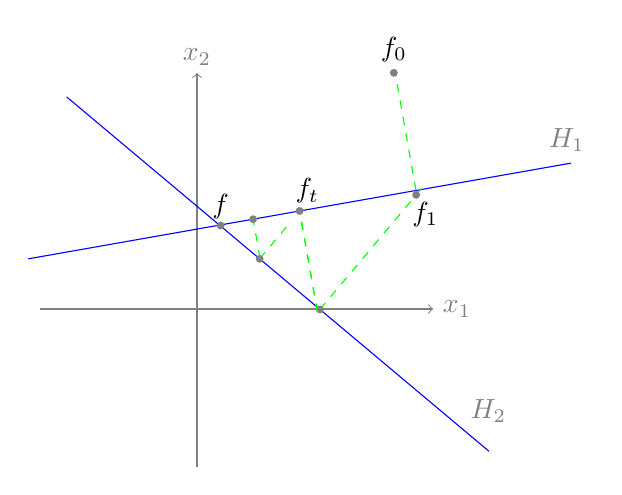
\begin{tikzpicture}
	
	\draw [gray] [->](-2,0) -- (3,0); % x-Achse
	\draw [gray] (3, 0) node [right] {$x_1$};
	
	\draw [gray] [->](0,-2) -- (0,3); % y-Achse
	\draw [gray] (0, 3.2) node {$x_2$};
	
	\draw [rotate=-40, xshift=1cm, yshift=1cm] [blue] (3,0) -- (-4,0); % blue ray	
	\draw [gray, xshift=3.7cm, yshift=-1.3cm] (0,0) node {$H_2$};
	
	\draw [rotate=10, xshift=1cm, yshift=1cm] [blue] (4,0) -- (-3,0); % blue ray
	\draw [gray, rotate=10, xshift=5cm, yshift=1.3cm] (0,0) node {$H_1$};
	
	\draw [rotate=100, xshift=1cm, yshift=-3cm, dashed] [green] (0,0) -- (1.5,0); % green from strat
	\fill[color=gray, xshift=1cm, yshift=3cm] (1.5,0) circle (0.05cm); % f point
	\draw [color=black, xshift=1cm, yshift=3cm] (1.5,0.3) node {$f_0$};
	
	\draw [rotate=50, xshift=1cm, yshift=-1.2cm, dashed] [green] (0,0) -- (2,0); % green from strat
	\fill[color=gray,rotate=50, xshift=1.4cm, yshift=-1.2cm] (1.5,0) circle (0.05cm); % f 1 point
	\draw [color=black,xshift=1.4cm, yshift=1.2cm] (1.5,0) node {$f_1$};
		
	\draw [rotate=100, xshift=-0.3cm, yshift=-1.5cm, dashed] [green] (0,0) -- (1.3,0); % green from strat	
	\fill[color=gray,rotate=50, xshift=1cm, yshift=-1.2cm] (0,0) circle (0.05cm); % f 2 point
	%\draw [color=black, xshift=1.45cm, yshift=-0.2cm] (0,0) node {$f_2$};
		
	\draw [rotate=100, xshift=-0.3cm, yshift=-1.5cm, dashed] [green] (0,0) -- (1.3,0); % green from strat	
	\fill[color=gray,rotate=100, xshift=-0.3cm, yshift=-1.5cm] (1.3,0) circle (0.05cm); % f 3 point
	\draw [color=black, xshift=0.1cm, yshift=1.5cm] (1.3,0) node {$f_t$};
	
	\draw [rotate=50, xshift=0.3cm, yshift=-0.2cm, dashed] [green] (0.7,0) -- (1.3,0); % green from strat		
	\fill[color=gray, rotate=50, xshift=0.3cm, yshift=-0.2cm] (0.7,0) circle (0.05cm); % f 4 point
	%\draw [color=black, xshift=0.1cm, yshift=0.3cm] (0.7,0) node {$f_4$};
	
	\draw [rotate=100, xshift=-0.2cm, yshift=-0.9cm, dashed] [green] (0.7,0) -- (1.3,0); % green from strat	
	\fill[color=gray, rotate=100, xshift=-0.2cm, yshift=-0.9cm] (1.2,0) circle (0.05cm); % f point
	
	\fill[color=gray, xshift=0.3cm, yshift=1.06cm] (0,0) circle (0.05cm); % f point
	\draw [color=black, xshift=0.3cm, yshift=1.3cm] (0,0) node {$f$};	
	
	\end{tikzpicture}
	\caption{Eine Veranschaulichung der Arbeitweise des Kaczmarz-Verfahrens in $\R^2$.}
	\label{fig:3.10}
\end{figure}

\begin{Bemerkung}
	Die Abbildung \ref{fig:3.10} zeigt ein Fall, wo die Lösung immer gefunden werden kann, denn der Schnittpunkt zweier Geraden ist immer exakt bestimmbar. Schon ab $\R^n$ für $n \geq 2$ ändert sich die Situation in den realen Fällen drastisch. Der Grund dafür ist, dass man ein mit Rauschen behaftetes System $Af \approx p + \epsilon$ hat. Somit ist jede Hyperebene $H_j$ um ein $\epsilon_j, \ j \in [1, n], \ n \in \N$ von dem Schnittpunkt verschoben. Das heißt, dass die Lösung $\tilde{f} \approx f$ in einem kleinem Toleranzvolumen $\prod \limits_{j=1}^{n}\epsilon_j$ liegt und daher nur annähernd angebbar ist.
	\label{be.:11}
\end{Bemerkung}

In \cite{Neufeld15} wird gezeigt, dass das randomisierte Verfahren eine schnellere Konvergenz nachweist. Aus diesem Grund werden wir dieses Vorgehen in Betracht ziehen. 
\begin{Definition}[Randomisierter Kaczmarz-Algorithmus]
	Sei $Af = p$ ein konsistentes, lineares Gleichungssystem. Sei $f_0 \in \R^m$ ein beliebiger Startwert. Für $t = 0, 1, 2, ...$ ist der Randomisierte Kaczmarz-Algorithmus definiert als
	\begin{equation}
			f_{t+1} = f_t + \frac{p_j - \langle a_j, f_t \rangle}{\parallel a_j \parallel_{2}^{2}}a_j,
			\label{equa:3.25}
	\end{equation}
	wobei $a_j$ die $j$-te Zeile von $A$ ist und $p_j$ die dazugehörige Projektion. $j$ wird zufällig ausgewählt.
	\label{def:5}	
\end{Definition} 
Wir wollen nun (\ref{equa:3.25}) etwas besser verstehen. Dafür formen wir diese Gleichung etwas um und bekommen

\[f_{t+1} = f_t + \left( \frac{p_j}{\parallel a_j \parallel_{2}} - \langle \frac{a_j}{\parallel a_j \parallel_{2}}, f_t \rangle \right) \frac{a_j}{\parallel a_j \parallel_{2}}.\]

Der eingeklammerte Teil der Gleichung stellt den Abstand von $f_t$ zu der $j$-ten Hyperebene $H_j$ in der Hesseschen Normalform Darstellung dar. Die Multiplikation mit $\frac{a_j}{\parallel a_j \parallel_{2}}$ liefert die Orthogonalität zu der $H_j$. Somit haben wir die oben beschriebene Lotprojektion, oder auch orthogonale Projektion auf $H_j$ genannt. 

Nun wollen wir uns von der Qualität des Verfahrens überzeugen, dessen genaue Implementierung in \ref{cha:A.5} (insbesondere die Abbruchbedingung (\ref{equa:A.1}) des Verfahrens) erläutert ist. Dazu sei die Abbildung \ref{fig:3.11} betrachtet. Die Ergebnisse in der Abbildung \ref{fig:3.11} wurden unter den gleichen Bedingungen, wie für die gefilterte Rückprojektion in den Abbildungen \ref{fig:3.6} für ungestörte und \ref{fig:3.8} (mittig) für gestörte Daten erzeugt. 

Man erkennt, dass die Ergebnisse der iterativen Rekonstruktion optisch gleichviel (oder sogar mehr) Informationsgehalt bieten, wie die der gefilterten Rückprojektion.
\begin{figure}[!h]
	\begin{center}
		\subfloat[\label{fig:3.11.a}Iterative Rekonstruktion aus nicht verrauschten Daten von \ref{fig:3.2.b}.]{{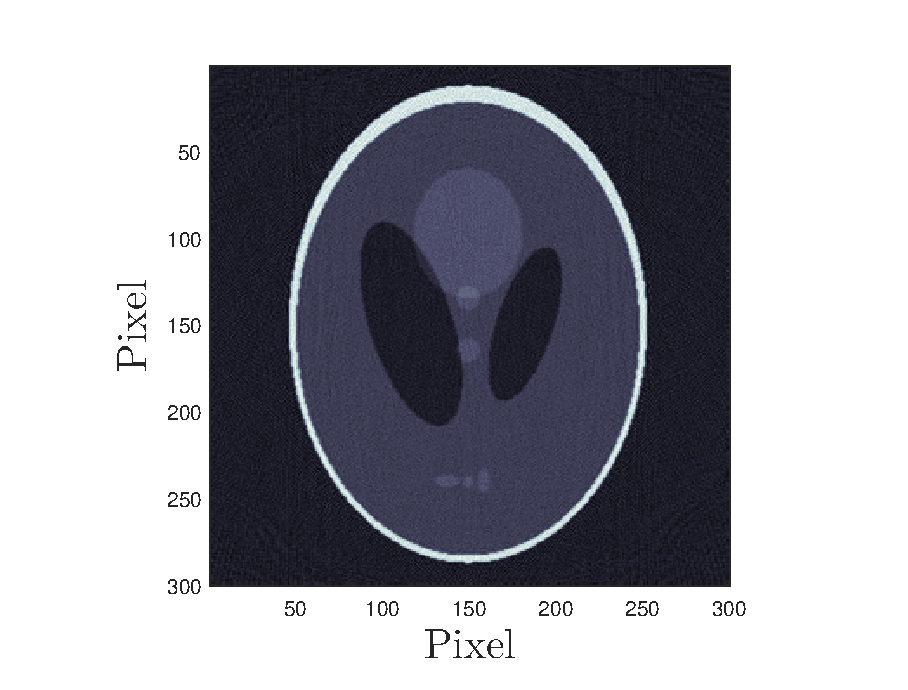
\includegraphics[width=0.5\textwidth]{iter.eps} }}
		\subfloat[\label{fig:3.11.b}Iterative Rekonstruktion aus verrauschten Daten von \ref{fig:3.7.b}]{{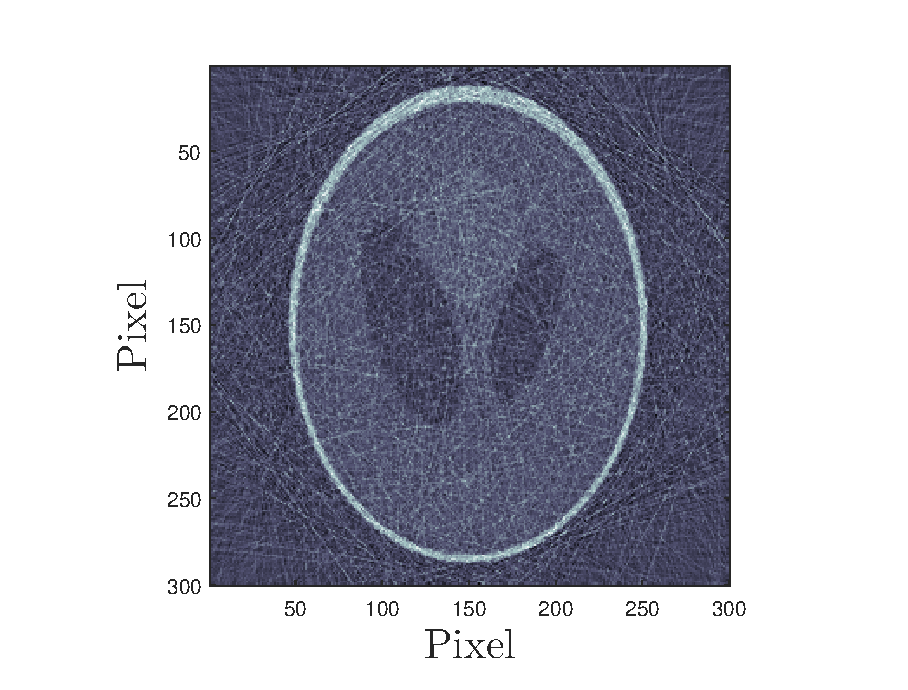
\includegraphics[width=0.5\textwidth]{iterNoised.eps} }}
	\end{center}
	\caption{Randomisierte iterative Rekonstruktionen (a) nicht verrauscht, (b) verrauscht. Die Projektionen in Beiden Fällen wurden für alle Winkel $\theta$ von $1^{\circ}$ bis $180^{\circ}$ mit der Schrittweite von $1^{\circ}$ berechnet. Detektorbreite ist $k=300$.}
	\label{fig:3.11}
\end{figure}

Jetzt wollen wir experimentell an einem Beispiel nachweisen, dass das randomisierte Verfahren in der Tat schneller konvergiert als das vorwärts projektive. Für unsere Testzwecke wählen wir ein Phantombild mit der Größe $50\times50$ Pixel (\MATLAB, \verb|phantom(50)|). Die kleine Größe des Phantombildes soll die Größe der Systemmatrix in annehmbaren Rahmen halten, da sonst zu große Matrizen entstehen, die sehr lange Rechenzeiten brauchen werden. Schließlich wollen wir nur die Konvergenz des Verfahrens untersuchen.
\begin{figure}[!h]
	\begin{center}
		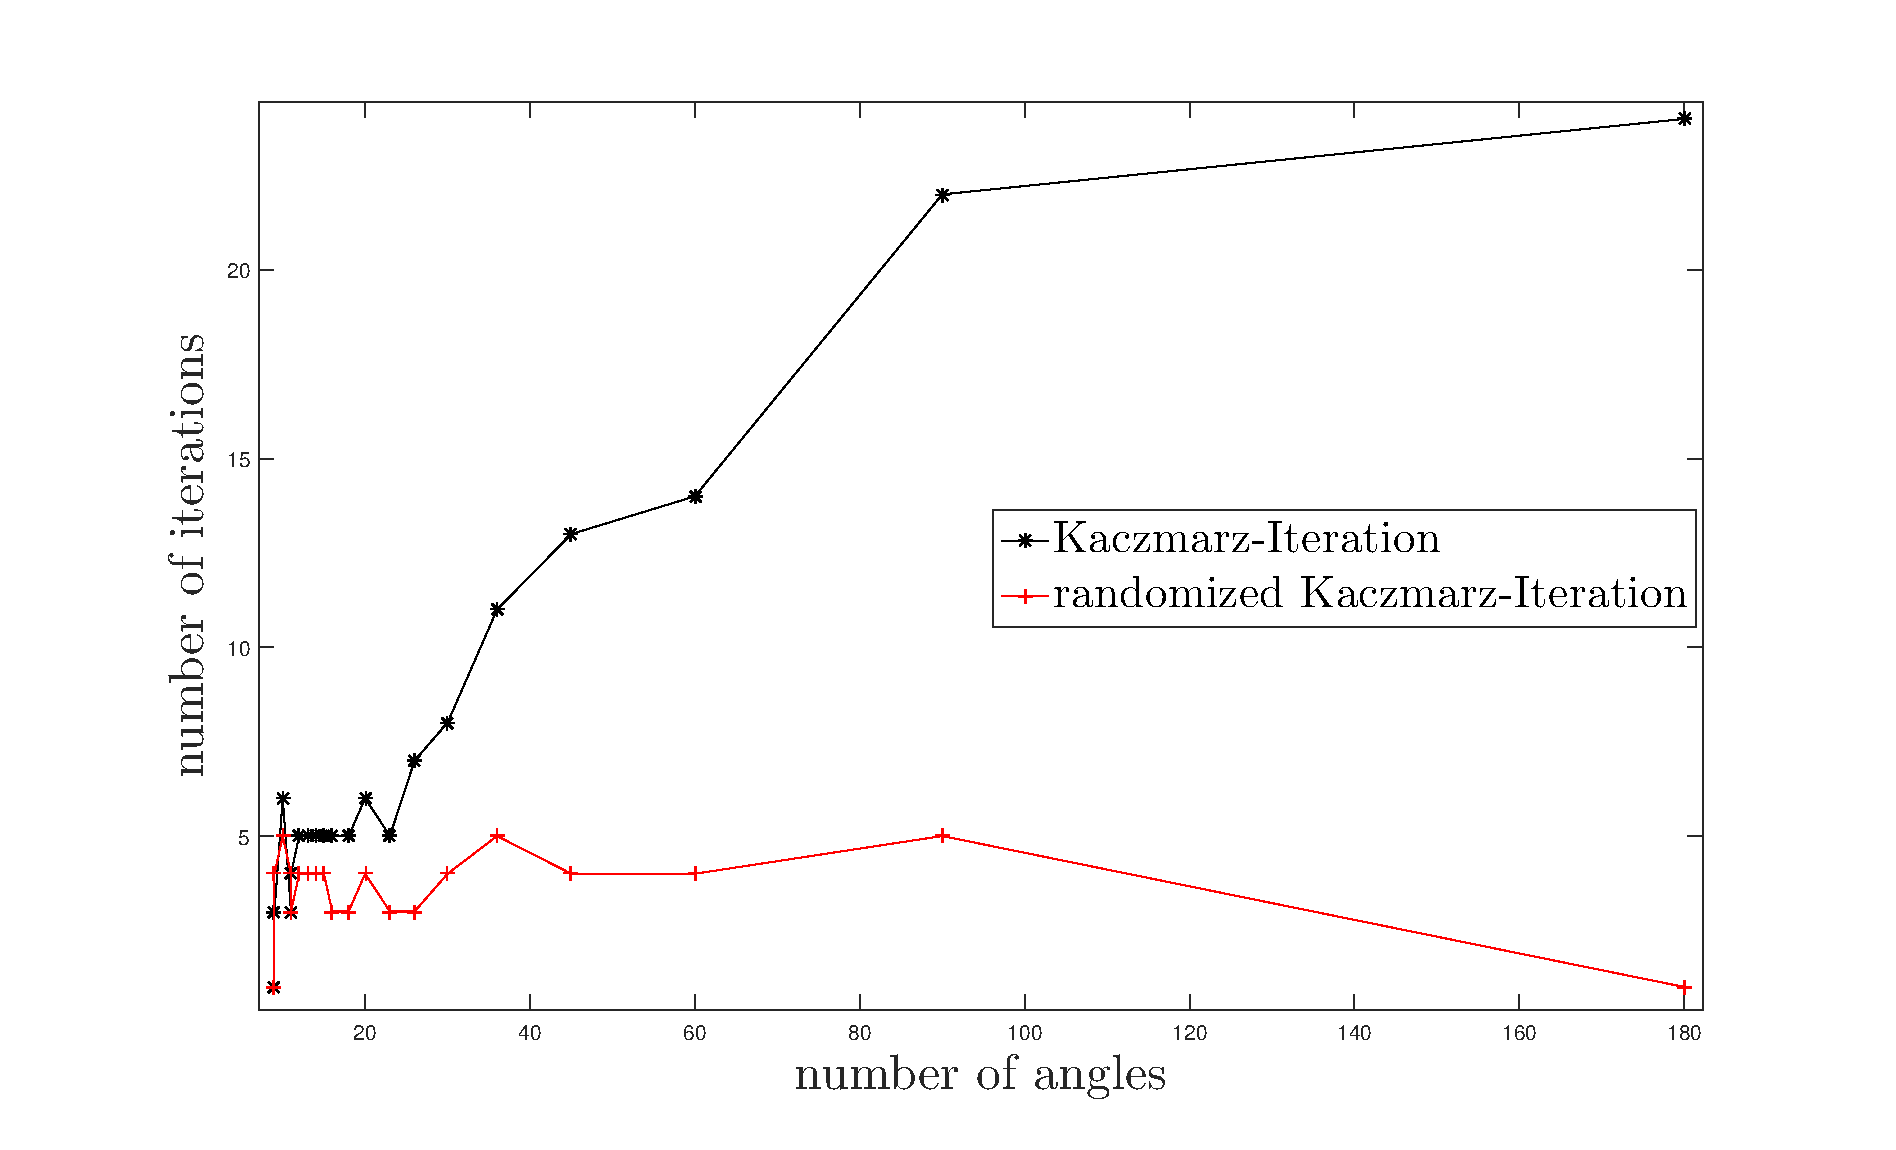
\includegraphics[width=\textwidth]{iterVSforward.eps}
	\end{center}
	\caption{Ein Vergleich des randomisierten und vorwärts projektiven Kaczmarz-Verfahrens. Der Test wurde für die Rekonstruktion eines $50 \times 50$ Pixel großen Bildes durchgeführt. In jedem Testschritt wurde die Winkelanzahl erhöht, sodass die Systemmatrix immer größer wurde.}
	\label{fig:3.12}
\end{figure}

In der Abbildung \ref{fig:3.12} ist das Ergebnis des Tests aus verrauschten (Salzstreuer-Effekt) Daten zu sehen. Dabei wurde die Systemmatrix in jedem Testschritt vergrößert, indem sich die Winkelanzahl und somit die Projektionsanzahl erhöhten. Der erste Testschritt wurde mit einer Winkelschrittweite von 20°, also für $q = 9$ Winkelpositionen durchgeführt. Die Detektorbreite wurde mit $k = 50$ initialisiert, was insgesamt für $A \in \R^{450\times2500}$ im erstem Testschritt ergeben hat. Der Test wurde bis $q = 180^{\circ}$ mit der Winkelschrittweite von 1°, das heißt bis $A \in \R^{9000 \times 2500}$ durchgeführt.

Die Abbruchbedingung musste für jeden Testschritt angepasst werden, da die Größe von $A$ schrittweise erhöht wurde und damit auch die Fehleranfälligkeit des Verfahrens. Aus (\ref{equa:A.1}) folgt $\delta = \alpha\epsilon$, wo $\epsilon = ||p - \tilde{p}||_2$ der Norm des Fehlers. $\alpha$ wurde als Verhältnis der Zeilenanzahl von $A$ im jetzt-Schritt zu davor-Schritt multipliziert mit dem Verhältnis der Winkelanzahl im jetzt-Schritt zu davor-Schritt aufgefasst. Da die Abbruchbedingung für beide Verfahren gleich war, kann man den Test als fair annehmen.

\subsection*{Rekonstruktion durch SWZ}
\label{cha:3.2.2}

Das letzte Verfahren, das wir uns anschauen werden beruht auf der Singulärwertzerlegung einer Matrix. Bekanntlich besitzt jede Matrix $A \in \R^{n\times}$ (wir beschränken uns hier auf reelle Matrizen) mindestens eine SWZ, sodass $A = U\Sigma V^{*}$ geschrieben werden kann. $U \in \R^{m\times m}$ ist die \textit{unitäre} Matrix des Bildes von $A$, $\Sigma \in \R^{m \times n}$ beinhaltet die Singulärwerte von $A$ auf der Diagonale sonst überall Null und $V^*$ ist die adjungierte der unitären Matrix des Kerns von $A$. Somit lässt sich die Gleichung (\ref{equa:3.22}) in der Form 
\begin{equation}
	Af = (U\Sigma V^*)f = p
	\label{equa:3.26}
\end{equation}
schreiben. Aus der Definition der unitären Matrizen folgt $U^{-1} = U^*$ und $(V^*)^{-1} = (V^*)^* = V$. Da $\Sigma$ eine Diagonalmatrix mit Singulärwerten größer Null ist, kann $\Sigma$ wie folgt invertiert werden
\begin{equation}
	\Sigma^+ = \left\{ \begin{matrix} \frac{1}{\sigma_{ji}} & : & \mbox{falls} \ j = i \\ 0 & : & \mbox{sonst} \end{matrix}\right. .
	\label{equa:3.27}
\end{equation}
Somit kann die Gleichung (\ref{equa:3.26}) invertiert werden, also
\begin{equation}
	f = (V\Sigma^+ U^*)p.
	\label{equa:3.28}
\end{equation}
Schreibt man die Gleichung \ref{equa:3.28} in expandierter Form auf
\begin{equation}
	f_i = \sum\limits_{i = 1}^{m}[\Sigma^+]_{ii} \langle p, u_i \rangle v_i,
	\label{equa:3.29}
\end{equation}
was mit $[\Sigma^+]_{ii} = \sigma^{-1}_{i}$ genau (\ref{equa:2.3}) entspricht. 

Mit den Ergebnissen aus dem Kapitel \ref{cha:2} wissen wir, dass bereits kleine Fehler in dem Messprozess stark oszillierend auf die Lösung (\ref{equa:3.29}) wirken können. Somit bedarf es einer Regularisierung in der Rekonstruktion. Wir werden die \textit{Tikhonov\footnote{Andrei Nikolajewitsch Tichonow (1906-1993) russischer Mathematiker.}-Regularisierung} benutzen, die wie folgt aufgeschrieben werden kann:
\begin{equation}
	d_i = \frac{\sigma_i}{\lambda^2 + \sigma_i^2}.
	\label{equa:3.30}
\end{equation}
Man erkennt, dass die Regularisierung für $\lambda = 0$ keine Wirkung ergibt. Ist $\lambda \geq 0$ so wirkt die Regularisierung dämpfend auf $\sigma_i$ und verhindert bei großen Werten die Oszillation der Lösung. Wir ersetzen die Elemente auf der Diagonale von $\Sigma^+$ mit (\ref{equa:3.30}) und benennen die Matrix mit $D$
\begin{equation}
	\tilde{f}_i = \sum\limits_{i = 1}^{m}[D]_{ii} \langle p, u_i \rangle v_i.
	\label{equa:3.31}
\end{equation} 

Wir wollen unsere Untersuchungen an dem Phantom-Beispiel (\verb|phantom(50)|) weiterführen. Wie in dem vorherigen Abschnitt werden die Daten mit dem Salzstreuer-Effekt beaufschlagt, sowie anschließend auch die Messdaten. Dabei wurden die Projektionen für 50 Winkel mit der Schrittweite von 3.6° aufgenommen. Folglich bekommt man eine Systemmatrix $A \in \R^{2500 \times 2500}$.

Nun wollen wir die Wirkung der Regularisierung (\ref{equa:3.31}) auf die Reihe (\ref{equa:2.4}) aus dem Satz \ref{satz:3} an unserem Beispiel verifizieren. Zunächst lassen wir das Verfahren (\ref{cha:A.6}) für verschiedene $\lambda$ das Phantombild rekonstruieren und tragen den entstandenen Rekonstruktionsfehler $||A\tilde{f} - p ||_2$ gegen $\lambda$ in einem Diagramm auf. Das Ergebnis ist in der Abbildung \ref{fig:3.13.a} zu sehen. Zu erkennen ist, dass der minimale Fehler etwa bei $\lambda_{min} = 5.5$ liegt (Abb. \ref{fig:3.13.a}). Anschließend lassen wir die Reihe (\ref{equa:2.4}) für zwei Parameter laufen, also $\lambda = 0$ und $\lambda_{min} = 5.5$. In der Abbildung \ref{fig:3.13.b} ist deutlich zu erkennen, dass die Reihe mit regularisierten Singulärwerten schneller konvergiert als die ohne Regularisierung.
\begin{figure}[!h]
	\begin{center}
		\subfloat[\label{fig:3.13.a}Der Fehler bei der Lösung durch SWZ in abhängigkeit von dem Regularisierungsparameter $\lambda$.]{{\includegraphics[width=0.5\textwidth]{svdErr.eps} }}
		\subfloat[\label{fig:3.13.b}Veranschaulichung der Konvergenz der Reihe (\ref{equa:2.4})]{{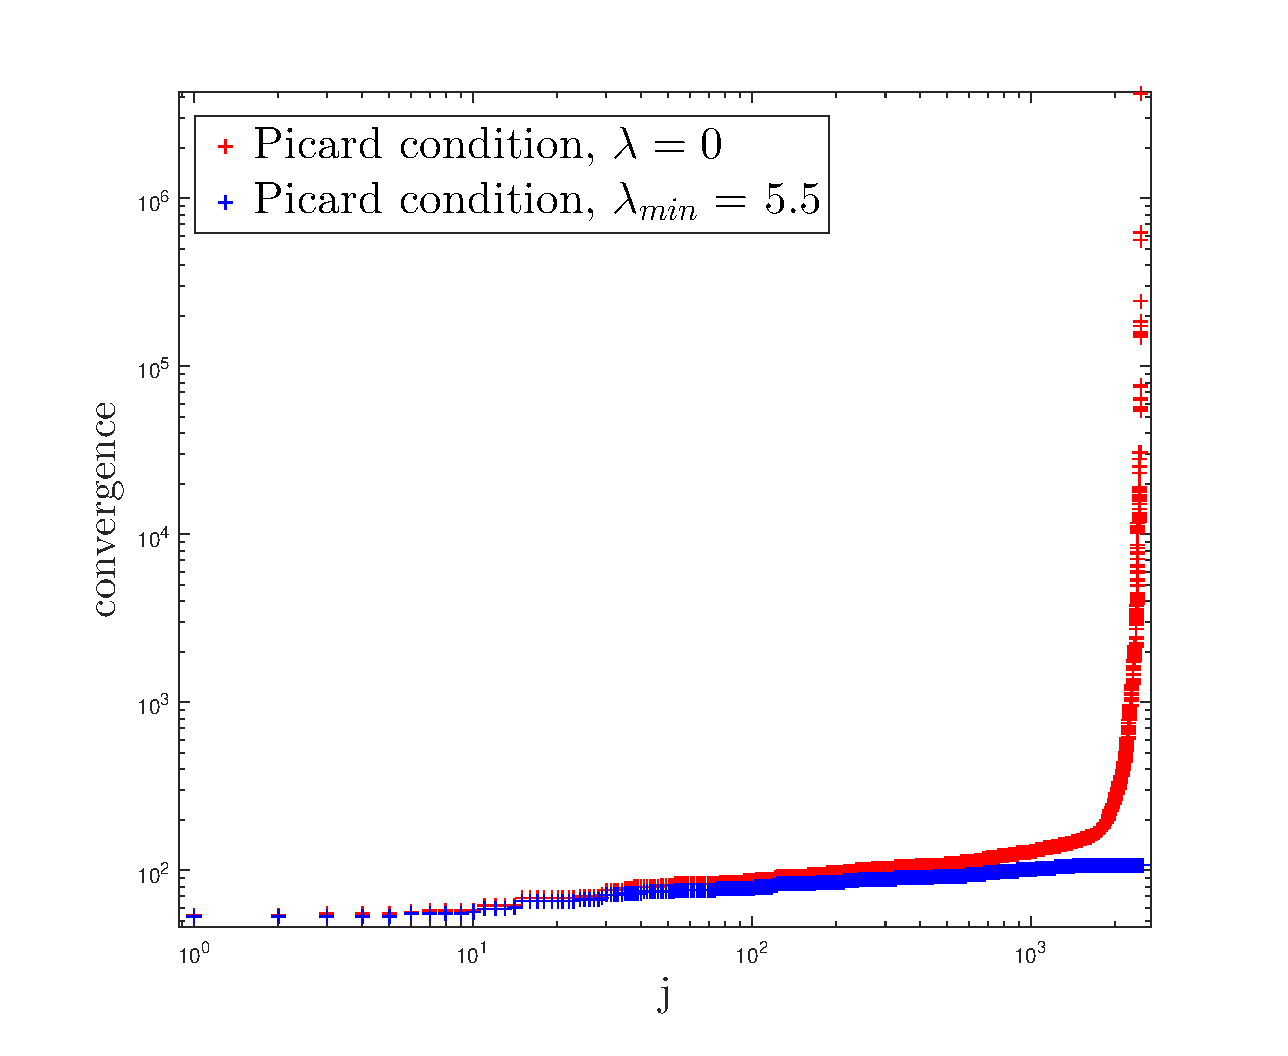
\includegraphics[width=0.5\textwidth]{picardIter.eps} }}
	\end{center}
	\caption{(a) Rekonstruktion durch SWZ, für ein Phantombild $(50\times50)$, Mit der Detektorbreite $k = 50$ und Winkelanzahl $q = 50$. (b) die  Konvergenz der Reihe (\ref{equa:2.4}) blau mit Regularisierung $\lambda_{min} = 5.5$ (das Minimum aus (a)), rot ohne Regularisierung.}
	\label{fig:3.13}
\end{figure}

\begin{figure}[!h]
	\centering
	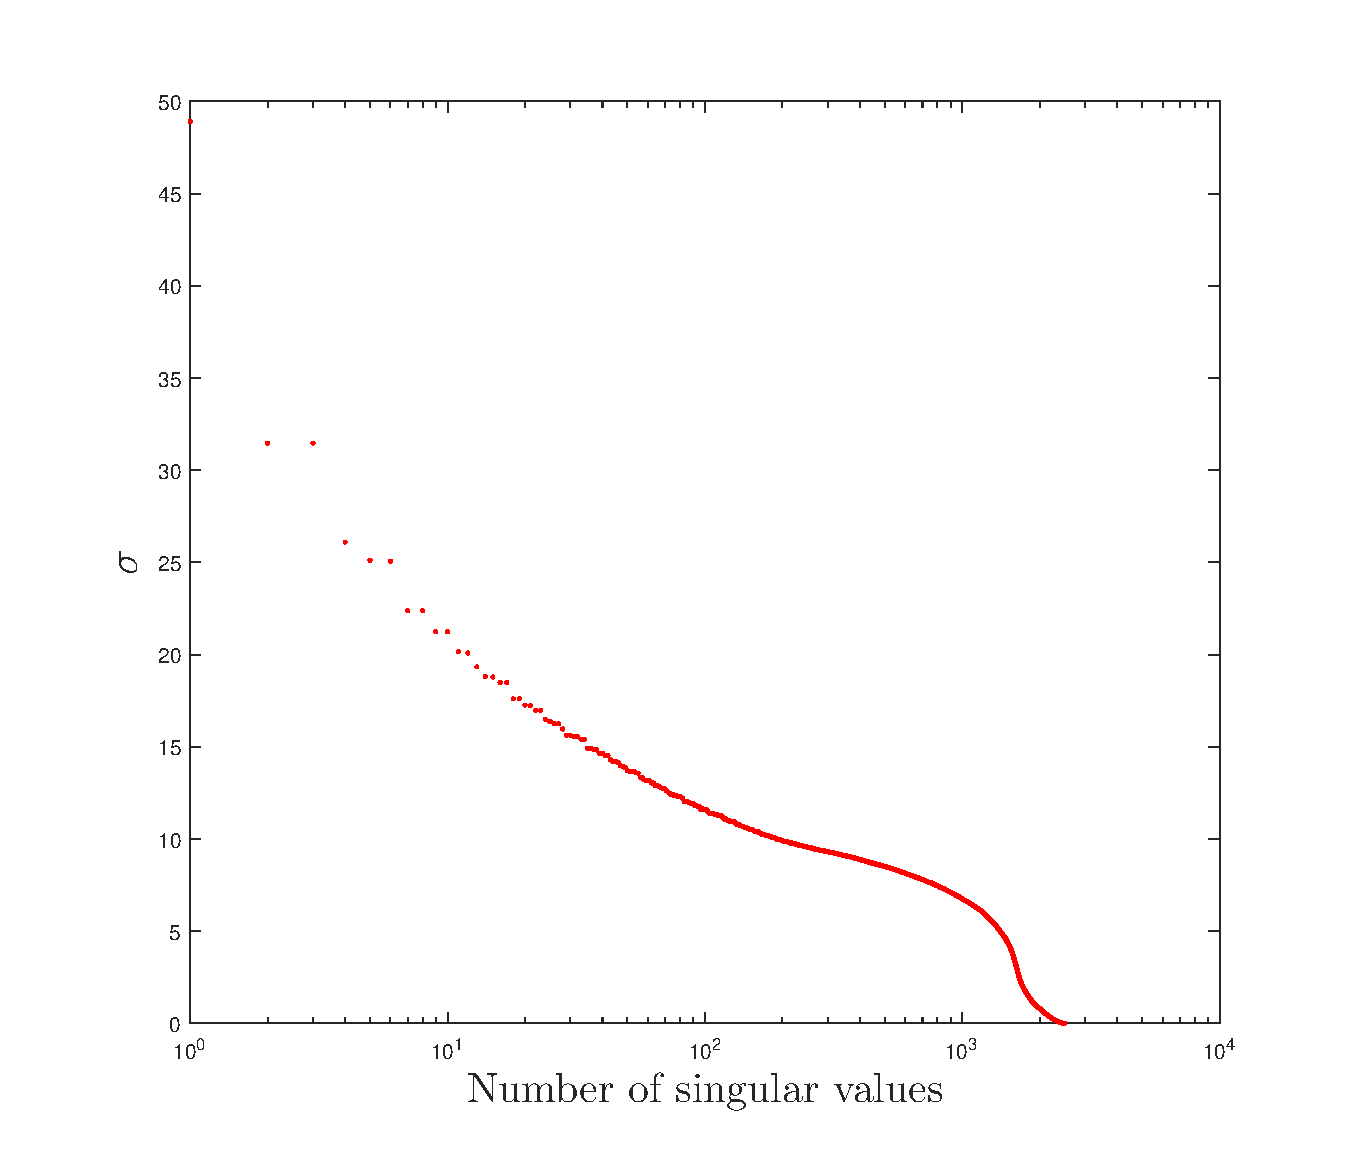
\includegraphics[width=0.5\textwidth]{singVal.eps}
	\caption{Die Folge der Singulärwerte für $A$ aus \ref{fig:3.13.a}}
	\label{fig:3.14}
\end{figure}

Insgesamt zeigt die Abbildung \ref{fig:3.13.b} die Schlechtgestelltheit des hier betrachten Problems $Af = p$ an einem konkreten Beispiel auf. Wir wissen, dass die Pcard-Bedingung (\ref{satz:3}) einen schnellen Abfall der Fourier-Koeffizienten $\langle p, u_i \rangle$ fordert, was eine stabile Lösung garantieren würde. Jedoch ist das bei Kompakten Operatoren, wie $\mathcal{R}$ ist es nie der Fall. Der Grund ist die SWZ, bei der die Singulärwerte eine abfallende Folge bilden (Abb. \ref{fig:3.14}). Was natürlich bei sehr kleinen Singulärwerten die Konvergenz der Reihe nicht fördert. Konvergiert die Reihe nicht, heißt das, dass die gemessenen Projektionen nicht in dem Bild der Operators $\mathcal{R}$ liegen. Was im Falle der verrauschten Daten garantiert ist. Durch eine passende Regularisierung ($\lambda = 5.5$) verschiebt man die verfälschten Fourier-Koeffizienten in die richtige Richtung und bekommt damit eine Minimum-Norm-Lösung. Was hier wieder zu der Abbildung \ref{fig:3.13.a} führt. Die Wirkung der Regularisierung ist in der Abbildung \ref{fig:3.15} offensichtlich.
\begin{figure}[!h]
	\centering
	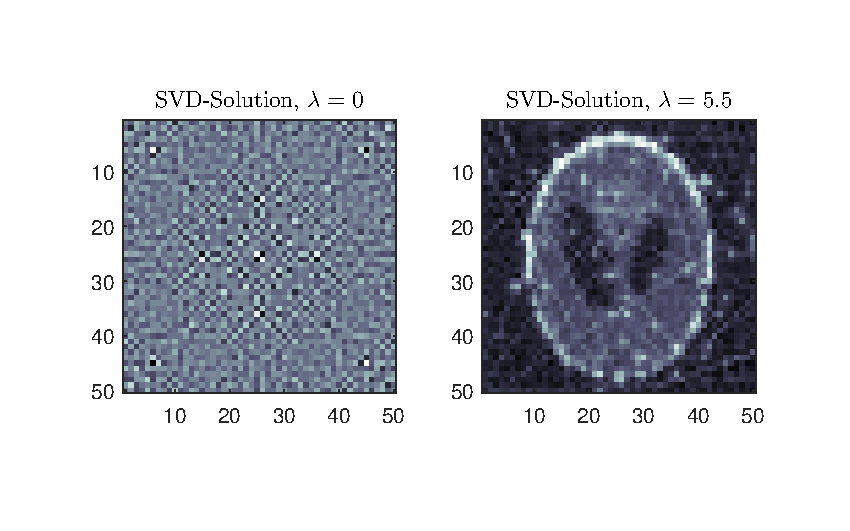
\includegraphics[width=\textwidth]{svdRedANDnotReg.eps}
	\caption{Die Rekonstruktion des Phantombildes mit der Größe $50\times50$ Pixel. Links nicht regularisiert $\lambda = 0$, recht Regularisierung mit $\lambda=5.5$.}
	\label{fig:3.15}
\end{figure}

Es ist natürlich sehr aufwendig, das Verfahren für verschiedene $\lambda$ rechnen zu lassen, um eine Minimum-Norm-Lösung zu bekommen. In der Praxis gibt es ein heuristisches Verfahren mit dem man ein optimales $\lambda_{opt}$ bestimmen kann. In der Abbildung (\ref{fig:3.14}) sehen wir, dass die Folge des Singulärwerte etwa bei $10^3$ einen Knick nach unten macht, die Singulärwerte in diesem Bereich haben den Wert zwischen 4-6. Setzt man diese Werte für $\lambda$ zu Regularisierung ein, so liefert das Verfahren die Minimum-Norm-Lösung.